\documentclass[11pt,a4paper]{article}

\usepackage[margin=2.5cm]{geometry}
\usepackage[T1]{fontenc}
\usepackage[utf8]{inputenc}
\usepackage{lmodern}
\usepackage{amsmath,amssymb}
\usepackage{booktabs}
\usepackage{tikz}
\usepackage{longtable}
\usepackage{array}
\usepackage{enumitem}
\usepackage{calc}
\usepackage{graphicx}
\usepackage{fvextra}
\usepackage{microtype}
\usepackage[colorlinks=true,linkcolor=black,citecolor=black,urlcolor=blue]{hyperref}

% --- float placement: keep float pages top-aligned, defer less eagerly ---
\makeatletter
\setlength{\@fptop}{0pt}
\makeatother
\renewcommand{\topfraction}{0.9}
\renewcommand{\bottomfraction}{0.8}
\renewcommand{\textfraction}{0.07}
\renewcommand{\floatpagefraction}{0.75}

\providecommand{\tightlist}{\setlength{\itemsep}{0pt}\setlength{\parskip}{0pt}}

\title{LLM-Based Agentic Monitoring vs.\ Classical Change-Point Detection for
Financial Market Regime Identification}
\author{Oscar Pham \& Paul Chen}
\date{\today}

\begin{document}
\maketitle

\begin{abstract}
We present a preregistered experiment comparing an LLM-based agentic monitoring system to a suite of classical change-point detectors for identifying regime breaks in two quantitative trading strategies. In this experiment, the agentic system integrates a small language model (qwen2.5:1.5b with grammar-constrained decoding) with filtered financial news, macroeconomic vintages, and strategy telemetry through a triage-escalation architecture. The classical statistical detection layer uses Page-Hinkley, BOCPD, HMM, and distributional threshold detectors.

We compare the two arms on identical point-in-time data across 12 historical windows (2004--2020), evaluating detection latency, false-positive rate (FPR), and recall for two strategies: statistical arbitrage and cross-sectional momentum.

The historical windows were divided into a development and a test set. On the development set (8 event-window pairs), the agentic system detects regime shifts 9.75 days earlier on average, with recall of 8/8 compared to 6/8 from classical. The confirmatory test set (5 event-window pairs) shows a directionally consistent latency advantage of 4.4 days (p = 0.25, n = 5). The results provide suggestive but not confirmatory evidence that multi-signal LLM fusion reduces detection latency relative to classical statistical methods.
\end{abstract}
% ============================================================
\section{Introduction}\label{sec:intro}

\subsection{Motivation}\label{sec:motivation}

Quantitative trading strategies are subject to regime breaks. The August 2007 quant meltdown (Khandani \& Lo, 2007), the 2009 momentum crash (Daniel \& Moskowitz, 2016), and the February 2018 volatility event demonstrate that such breaks can destroy years of accumulated profit within days. Monitoring for regime transitions is therefore a first-order operational concern.

Classical change-point detection methods such as Page-Hinkley (1954), Bayesian online change-point detection (Adams \& MacKay, 2007), hidden Markov models (Hamilton, 1989), and threshold-based approaches operate exclusively on the strategy's return stream. They are theoretically well-founded but react only after the statistical properties of the stream have already shifted, introducing unavoidable detection latency.

Recent advances in large language models (LLMs) suggest an alternative: a system that fuses statistical telemetry with natural-language context (news, macroeconomic releases, market commentary) to anticipate or accelerate regime identification. If news coverage of a developing crisis precedes its statistical manifestation in strategy returns, an LLM-based monitor might detect regime breaks earlier.

\subsection{Hypotheses}\label{sec:hypotheses}

This paper reports a preregistered experiment testing three hypotheses:

\begin{itemize}
\tightlist
\item \textbf{H1 (co-primary):} The agentic monitoring system achieves both lower detection latency AND lower false-positive rate than the best classical detector.
\item \textbf{H2:} Any agentic advantage generalises across both strategies.
\item \textbf{H3:} The magnitude of advantage differs by strategy.
\end{itemize}

\subsection{Contributions}\label{sec:contributions}

\begin{enumerate}
\tightlist
\item \textbf{A monitoring architecture.} A three-layer agentic monitor fusing strategy telemetry, filtered financial news, and macroeconomic vintages through a triage-escalation pipeline, using a 1.5B-parameter language model with grammar-constrained decoding on consumer hardware.
\item \textbf{An evaluation protocol with strict information parity.} Both arms observe only information available on each decision date, on a survivorship-bias-free universe built from historical constituent membership intervals, a distinction that reverses the sign of the anchor event ($+3.4\%$ on a survivor-only universe against a $-4.8\%$ drawdown point-in-time).
\item \textbf{A memorisation bound.} A three-condition leakage harness (standard, date-masked, synthetic) separating genuine detection from recall of famous events.
\item \textbf{Full disclosure of deviations and operational failure modes}, including news-agent failure rates and triage-gate saturation.
\end{enumerate}

\subsection{Summary of Findings}\label{sec:summary}

We find that the agentic system detects regime breaks significantly earlier on the development set (9.75 days, Holm-adjusted p = 0.0156), but that the confirmatory test set is underpowered to confirm this finding (5 event pairs yield a minimum achievable p = $\frac{1}{32}$ under exact permutation). The FPR co-primary endpoint does not favour the agentic arm on either set; on the test set the agentic arm exhibits higher FPR than classical. We trace the latency advantage to news coverage preceding statistical manifestation in returns, and the FPR result to saturation of the sentiment-based triage gate, which routes nearly every day with available news to full inference.

% ============================================================
\section{Data}\label{sec:data}

All inputs are constructed point-in-time (PIT): on any decision date $t$, both
arms observe only values that were published on or before $t$. This section
documents each input stream, its temporal coverage, and the coverage gaps that
constrain the window partition in Section~\ref{sec:protocol}.

\subsection{Point-in-Time Universe Construction}\label{sec:data-universe}

The eligible security universe is reconstructed from historical S\&P 500
constituent membership intervals. Each interval records the date on which a
security entered the index and, where applicable, the date on which it left,
so that securities subsequently delisted, acquired, or removed remain eligible
for the periods during which they were actual members. At each monthly
rebalance, only securities whose membership interval contains the rebalance
date are admitted.

This yields approximately 347 eligible names per month, against approximately
542 under a survivor-only universe constructed from present-day index
membership. Sleeves are built by \texttt{scripts/build\_pit\_sleeves.py}, with
each sleeve masked to the membership intervals in force on the relevant date.

\subsection{Strategy Return Series}\label{sec:data-pnl}

Two daily profit-and-loss series are constructed on the PIT universe: AL\_PCA
(Avellaneda--Lee statistical arbitrage), spanning 2003--2014, and JT\_MOM
(Jegadeesh--Titman cross-sectional momentum), spanning 2003--2020 and computed
from position-level returns on the PIT candidate pool. Construction details are
given in Section~\ref{sec:method-strategies}.

The two series are close to statistically independent, with a daily return
correlation of approximately $0.003$. This near-orthogonality is what makes the
cross-strategy hypotheses (H2, H3) informative: the strategies break on
different events, so an advantage observed on both is unlikely to reflect a
single shared shock.

\textbf{Coverage gap.} The AL\_PCA curve does not extend beyond 2014, excluding
AL\_PCA from three of the four test-set event windows. This reduces the
confirmatory sample to five event pairs and contributes directly to the power
limitation analysed in Section~\ref{sec:power}.

\subsection{News and Macroeconomic Inputs}\label{sec:data-context}

Natural-language context is drawn from the FNSPID financial news dataset:
approximately 11.8~million articles totalling 22~GB, stored as per-year Parquet
files and indexed by publication date. On each decision date the news agent
queries a 7-day trailing window and applies a risk-term filter, so that no
article published after the decision date can enter the context.

\textbf{News-corpus density variation.} The FNSPID store covers 2003--2020 (11.8\,M articles after non-English filtering), so all evaluation windows
  receive news context. However, article density is uneven: the 2007--2016 core averages ${\sim}2{,}800$ articles/day, while 2003--2006 is sparse
  (${\sim}80$/day, mostly wire headlines) and 2017--2020 is intermediate
  (${\sim}1{,}400$/day). The pre-2009 rows are predominantly a Russian
  general-news scrape with empty tickers (Lenta.ru); the NYT Archive API
  supplements these early windows with English-language market coverage.
  Density variation does not affect classical detectors (which use only returns)
  but may modulate agentic sensitivity through the triage intensity-$z$ score.

  Macroeconomic context is retrieved from FRED/ALFRED via API. ALFRED vintage
  series are used rather than current-revision FRED series, so that each value
  reflects the figure as published on the decision date rather than after
  subsequent revision. Headline series such as GDP and payrolls are revised
  substantially, and a current-revision series would leak post-hoc information
  into the agentic arm that the classical arm never sees.

  \subsection{Coverage Summary}\label{sec:data-coverage}

  Table~\ref{tab:coverage} records which inputs are available for each evaluation
  window, and Figure~\ref{fig:timeline} shows the same information on a common
  time axis.

  \begin{table}[htbp]
  \centering
  \small
  \caption{Input availability by evaluation window. Macroeconomic vintages are
  available throughout. ``JT\_MOM only'' reflects the AL\_PCA curve ending in
  2014.}
  \label{tab:coverage}
  \begin{tabular}{llll}
  \toprule
  Window & Type & Strategy returns & News \\
  \midrule
  \multicolumn{4}{l}{\emph{Development set}} \\
  Calm 2004--2006      & Calm  & Both        & Yes \\
  Quant meltdown 2007  & Event & Both        & Yes \\
  GFC / Lehman 2008    & Event & Both        & Yes \\
  Momentum crash 2009  & Event & Both        & Yes \\
  Downgrade 2011       & Event & Both        & Yes \\
  Calm 2013--2014      & Calm  & Both        & Yes \\
  \addlinespace
  \multicolumn{4}{l}{\emph{Test set}} \\
  Flash crash 2010     & Event & Both        & Yes \\
  Calm 2012            & Calm  & Both        & Yes \\
  China devaluation 2015 & Event & JT\_MOM only & Yes \\
  Calm 2017            & Calm  & JT\_MOM only & Yes \\
  Volmageddon 2018     & Event & JT\_MOM only & Yes \\
  COVID-19 2020        & Event & JT\_MOM only & Yes \\
  \bottomrule
  \end{tabular}
  \end{table}

  \begin{figure}[htbp]
  \centering
  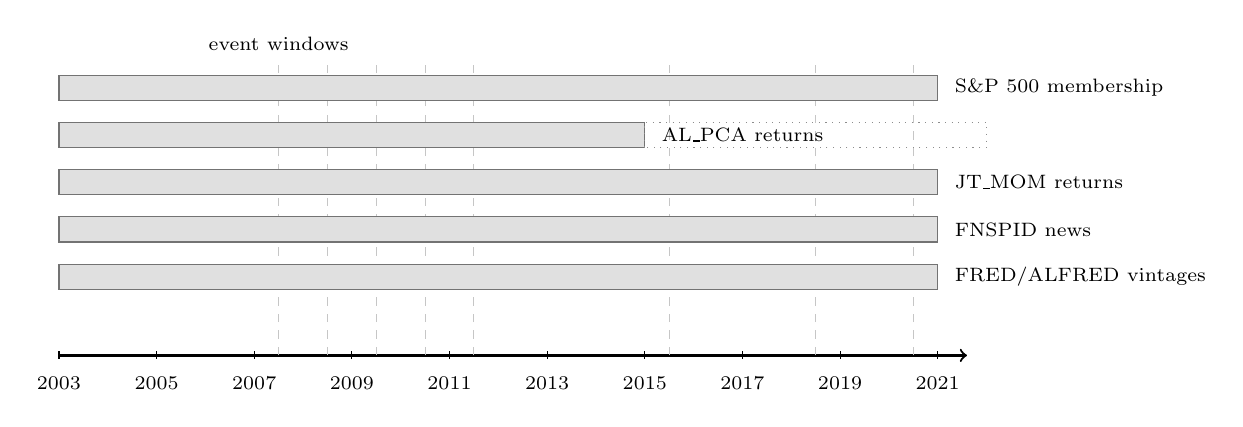
\begin{tikzpicture}[x=0.62cm, y=1cm]

  % ---- geometry: year 2003 at x=0 ... year 2021 at x=18 ----
  \def\ymin{2003}
  \def\ymax{2021}

  % ---- axis ----
  \draw[->, thick] (0,-0.4) -- (18.6,-0.4);
  \foreach \yr in {2003,2005,2007,2009,2011,2013,2015,2017,2019,2021} {
    \pgfmathsetmacro\xx{\yr-\ymin}
    \draw (\xx,-0.35) -- (\xx,-0.45);
    \node[font=\scriptsize, anchor=north] at (\xx,-0.55) {\yr};
  }

  % ---- event-window markers (drawn first, behind the bars) ----
  \foreach \yr/\lab in {2007/2007, 2008/2008, 2009/2009, 2010/2010,
                        2011/2011, 2015/2015, 2018/2018, 2020/2020} {
    \pgfmathsetmacro\xx{\yr-\ymin+0.5}
    \draw[gray!45, dashed] (\xx,-0.4) -- (\xx,3.3);
  }

  % ---- coverage bars: {y-position / start / end / label} ----
  \foreach \yy/\a/\b/\lab in {
      3.0/2003/2020/{S\&P 500 membership},
      2.4/2003/2014/{AL\_PCA returns},
      1.8/2003/2020/{JT\_MOM returns},
      1.2/2003/2020/{FNSPID news},
      0.6/2003/2020/{FRED/ALFRED vintages}} {
    \pgfmathsetmacro\xa{\a-\ymin}
    \pgfmathsetmacro\xb{\b-\ymin+1}
    \fill[black!12, draw=black!55] (\xa,\yy-0.16) rectangle (\xb,\yy+0.16);
    \node[font=\scriptsize, anchor=west] at (\xb+0.15,\yy) {\lab};
  }

  % ---- gaps: AL_PCA only ----
  \foreach \yy/\a/\b in {2.4/2014/2021} {
    \pgfmathsetmacro\xa{\a-\ymin+1}
    \pgfmathsetmacro\xb{\b-\ymin+1}
    \draw[black!45, dotted] (\xa,\yy-0.16) rectangle (\xb,\yy+0.16);
  }

  \node[font=\scriptsize, anchor=south] at (4.5,3.35) {event windows};

  \end{tikzpicture}
  \caption{Temporal coverage of each input stream, with evaluation event windows
  marked (dashed). Solid bars denote available coverage; dotted outlines denote
  periods for which an input is unavailable. The only binding constraint is the
  AL\_PCA return series, which ends in 2014 (PIT sleeves not built beyond that
  date); all other inputs cover the full 2003--2020
  evaluation span.}
  \label{fig:timeline}
  \end{figure}

% ============================================================
\section{Method}\label{sec:method}

\subsection{Trading Strategies}\label{sec:method-strategies}

\textbf{AL\_PCA.} Following Avellaneda and Lee (2010), we construct sector-sleeve
PCA-based mean-reversion portfolios on the PIT S\&P 500 universe. The first
$K = 15$ principal components per sector capture systematic factor exposure;
residuals are modelled as Ornstein--Uhlenbeck processes and traded when z-scores
exceed entry/exit thresholds.

\textbf{JT\_MOM.} Following Jegadeesh and Titman (1993), we rank PIT-universe
stocks by trailing 12-month returns (skipping the most recent month), go long
the top decile and short the bottom decile, and rebalance monthly. Daily PnL is
computed from position-level returns on the PIT candidate pool.

\subsection{Classical Arm}\label{sec:method-classical}

Four change-point detectors operate on the strategy's daily return stream
(Table~\ref{tab:detectors}). An aggregate classical alarm fires when 2 or more of
the 4 detectors fire within a 5 trading-day window, which reduces false positives
from individual noisy detectors at the cost of marginally increased latency. For
the primary H1 analysis the best single classical detector (HMM) is used as the
headline comparator, since the aggregation rule often underperforms the best
individual detector because of that latency penalty.

\begin{table}[htbp]
\centering
\footnotesize
\caption{Classical detectors. All operate on the daily return stream only.}
\label{tab:detectors}
\begin{tabular}{lll}
\toprule
Detector & Signal & Parameters \\
\midrule
Page-Hinkley (1954)        & Cumulative deviation from running mean & $\delta = 0.5$, $\lambda = 8.0$ \\
BOCPD (Adams \& MacKay, 2007) & Posterior mass on short run lengths & Hazard rate $1/250$ \\
HMM (Hamilton, 1989)       & Low- to high-volatility state transition & Two-state Gaussian, rolling \\
Distributional threshold   & Rolling z-score exceeds fixed threshold & Calibration-window z \\
\bottomrule
\end{tabular}
\end{table}

\subsection{Agentic Arm}\label{sec:method-agentic}
  The agentic monitoring system processes each trading day through a three-layer pipeline: \emph{triage}, \emph{news context agent}, and \emph{performance
  supervisor}. All layers share a common guardrail module that enforces
  information parity with the classical arm. The architecture is depicted in
  Figure~\ref{fig:architecture}.

  \begin{figure}[htbp]
  \centering
  \resizebox{\textwidth}{!}{%
  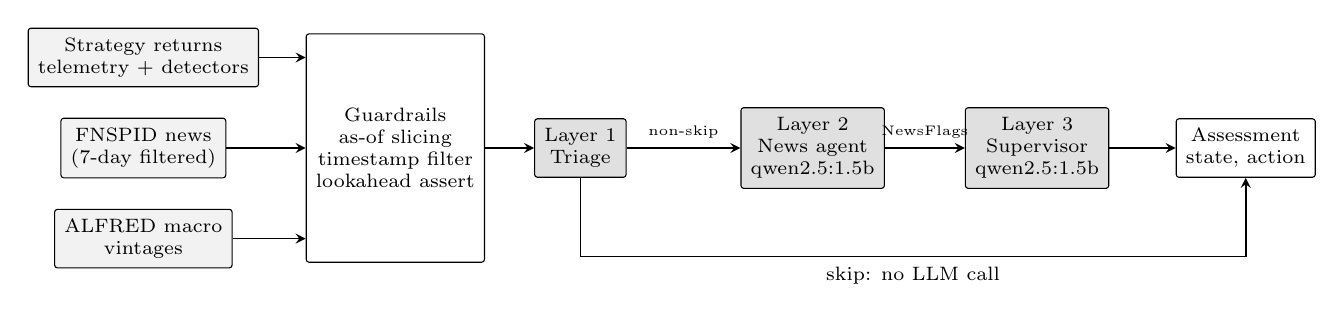
\begin{tikzpicture}[
    font=\scriptsize,
    box/.style={draw, rounded corners=1pt, align=center, inner sep=3.5pt},
    agent/.style={box, fill=black!12},
    arrow/.style={->, >=stealth, semithick}
  ]
  % inputs (stacked, left)
  \node[box, fill=black!5] (ret)   at (0, 1.15) {Strategy returns\\telemetry + detectors};
  \node[box, fill=black!5] (news)  at (0, 0.0)  {FNSPID news\\(7-day filtered)};
  \node[box, fill=black!5] (macro) at (0,-1.15) {ALFRED macro\\vintages};

  % guardrail module
  \node[box, minimum height=2.9cm] (guard) at (3.2, 0)
    {Guardrails\\as-of slicing\\timestamp filter\\lookahead assert};

  % pipeline
  \node[agent] (triage) at (5.55, 0) {Layer 1\\Triage};
  \node[agent] (na)     at (8.5, 0)  {Layer 2\\News agent\\qwen2.5:1.5b};
  \node[agent] (sup)    at (11.35, 0){Layer 3\\Supervisor\\qwen2.5:1.5b};
  \node[box]   (out)    at (14.0, 0) {Assessment\\state, action};

  \draw[arrow] (ret)   -- (guard.west |- ret);
  \draw[arrow] (news)  -- (guard);
  \draw[arrow] (macro) -- (guard.west |- macro);
  \draw[arrow] (guard) -- (triage);
  \draw[arrow] (triage) -- node[above, pos=0.5]{\tiny non-skip} (na);
  \draw[arrow] (na) -- node[above, pos=0.5]{\tiny NewsFlags} (sup);
  \draw[arrow] (sup) -- (out);
  \draw[arrow] (triage.south) -- ++(0,-1.0) -| node[pos=0.25, below]{skip: no LLM call} (out.south);
  \end{tikzpicture}%
  }
  \caption{Agentic monitoring architecture. All inputs pass through the
  fail-closed guardrail module before reaching the three-layer pipeline. The
  triage layer routes each trading day to \textsc{skip} (no LLM call) or to
  progressively richer inference modes.}
  \label{fig:architecture}
  \end{figure}

  \subsubsection{Layer 1: Triage}\label{sec:triage}

  The triage layer determines per-day computational budget by classifying each
  trading day into one of four modes based on three causal signals:

  \begin{enumerate}
    \item \textbf{FinBERT stress} ($s$): daily-maximum negative-sentiment
          probability from the ProsusAI FinBERT model applied to the day's
          filtered news headlines;
    \item \textbf{News intensity $z$-score}: causal, trailing-baseline
          $z$-score of regex risk-term hit counts across a 7-day trailing
          news window;
    \item \textbf{Classical detector count} ($n$): number of individual classical
          detectors that alarmed within 3 calendar days.
  \end{enumerate}

  \noindent The decision rule (fixed a priori, preregistration \S6.2) is:

  \[
  \text{mode} =
  \begin{cases}
  \textsc{classical\_escalation} & \text{if } \geq 2 \text{ detectors within 5 days (aggregate rule)} \\
  \textsc{thinking}              & \text{if } s \geq 0.60 \;\lor\; z \geq 2.0 \;\lor\; n \geq 1 \\
  \textsc{cheap}                 & \text{if } s \geq 0.30 \\
  \textsc{skip}                  & \text{otherwise}
  \end{cases}
  \]

  Days classified as \textsc{skip} incur no LLM call; the remaining modes proceed
  to the news agent and supervisor with progressively richer prompts.

  \subsubsection{Layer 2: News Context Agent}\label{sec:news-agent}

  For non-skip days, the news agent receives up to 40 articles from a 7-day
  trailing FNSPID query, filtered by a 23-term risk lexicon and sorted by
  risk-term density. It produces a structured \texttt{NewsFlags} JSON:

  \begin{itemize}
    \item \texttt{overall\_risk} $\in$ \{LOW, ELEVATED, HIGH, SEVERE\}
    \item \texttt{risk\_flags}: list of \{flag, evidence\} pairs
    \item \texttt{narrative}: free-text interpretation ($\leq$1500 chars)
    \item \texttt{confidence} $\in [0,1]$
  \end{itemize}

  \noindent Output is grammar-constrained via Ollama's \texttt{format=json}
  parameter with the schema passed at generation time. One repair retry is
  attempted on schema-validation failure (the validation error is appended to the
  prompt); persistent failures are logged and the day proceeds without news flags.

  \subsubsection{Layer 3: Performance Supervisor}\label{sec:supervisor}

  The supervisor receives a context packet assembled by the guardrail module:

  \begin{itemize}
    \item \textbf{Telemetry:} trailing 60-day mean return, volatility, cumulative
          return, current drawdown, worst single day all computed causally up to
          the decision date.
    \item \textbf{Detector alarms:} names and dates of classical detectors that
          have fired, filtered to $\leq$ \texttt{as\_of}.
    \item \textbf{Macro context:} ALFRED-vintage macro releases (GDP, payrolls,
          VIX, Treasury yields, TED spread) as published on the decision date.
    \item \textbf{News flags:} the Layer-2 output (when available).
  \end{itemize}

  \noindent The supervisor outputs a structured \texttt{AgentAssessment}:

  \begin{itemize}
    \item \texttt{state} $\in$ \{NORMAL, WATCH, ALERT, CRITICAL\}
    \item \texttt{action} $\in$ \{HOLD, INVESTIGATE, REDUCE, HALT\}
    \item \texttt{root\_cause}: free-text explanation ($\leq$1000 chars)
    \item \texttt{confidence} $\in [0,1]$
    \item \texttt{detectors\_cited}: classical detectors referenced
  \end{itemize}

  \noindent A day is counted as an \emph{alarm} if
  $\texttt{state} \in \{\text{ALERT}, \text{CRITICAL}\}$. Alarm clusters are
  de-duplicated with a 5-trading-day cooldown to match the classical aggregation
  rule.

  \subsubsection{Guardrails and Information Parity}\label{sec:guardrails}

  Four fail-closed guardrails enforce that the agentic arm never observes
  information unavailable to the classical arm on the same date:

  \begin{enumerate}
    \item \textbf{Causal context assembly} (\texttt{as\_of\_context}): telemetry
          and detector alarms are sliced to $\leq$ \texttt{as\_of}; no future
          returns enter the prompt.
    \item \textbf{Timestamp filter}: articles with publication date $>$
          \texttt{as\_of} are dropped.
    \item \textbf{Future-text scrub}: articles whose body text embeds any ISO
          date $>$ \texttt{as\_of} are dropped entirely.
    \item \textbf{Recursive lookahead assertion}: the complete context dictionary
          is scanned for any date string or timestamp object post-dating
          \texttt{as\_of}; violation raises a hard \texttt{LookaheadError}.
  \end{enumerate}

  \noindent Macroeconomic data uses ALFRED vintage series (first-print values) to
  avoid revision lookahead. For the pretraining-leakage harness (Condition~B), an
  additional date-masking pass replaces all ISO dates with a non-parseable
  sentinel (\texttt{XXXX-XX-XX}), preserving numerical evidence while blocking
  memorised event--date associations.

  \subsubsection{Model and Inference}\label{sec:model}

  Both agents use \textbf{qwen2.5:1.5b} served locally via Ollama with
  temperature $= 0$ (greedy decoding) and grammar-constrained JSON output. The
  model was selected after the preregistered choice (llama3.2:3b) failed
  structured-output benchmarks (11/30 valid JSON vs.\ 30/30 for qwen2.5:1.5b);
  the substitution was made before any evaluation data were examined
  (Deviation~1). Mean supervisor latency is 3--5\,s per trading day on the test
  hardware (RTX 3050 Ti, 4\,GB VRAM). Full prompt templates and hyperparameter
  justifications are given in Appendix~\ref{app:prompts}.

\subsection{Endpoints and Analysis Plan}\label{sec:method-endpoints}
All metrics, tests, and decision rules were specified before the evaluation freeze (\texttt{eval-freeze-v1} git tag). No thresholds were tuned on
  evaluation data.

  \subsubsection{Primary Endpoints}

  \paragraph{Detection latency.}
  For each event window, let $t_\text{onset}$ denote the preregistered onset date
  and $t_\text{alarm}$ the first alarm day (ALERT or CRITICAL for the agentic
  arm; the best single classical detector, HMM, for the classical arm,
  cf.\ Section~\ref{sec:method-classical}) falling in the detection zone
  $[t_\text{onset},\; t_\text{onset} + 21\text{d}]$. Latency is
  $\ell = t_\text{alarm} - t_\text{onset}$ in calendar days (negative values
  indicate early detection). A \emph{miss} (no alarm within the zone) is
  right-censored at $\ell = 21$ for all statistical tests, ensuring that
  non-detections contribute as worst-case latencies rather than being dropped.

  \paragraph{False-positive rate (FPR).}
  During calm windows, every alarm is a false positive. Agentic alarms are
  de-duplicated into \emph{cluster starts}: consecutive alarms within a
  5-trading-day cooldown are collapsed to a single event. FPR is then
  \[
    \text{FPR} \;=\; \frac{\text{cluster starts}}{\text{trading days}}
    \quad\text{(per calm window).}
  \]
  Classical FPR counts every alarm day without de-duplication. This
  asymmetry, documented as Deviation~9, biases in favour of the agentic arm;
  results should be interpreted accordingly.

  \subsubsection{Secondary and Exploratory Endpoints}

  \paragraph{Recall.}
  Binary per event window: $\text{detected} = 1$ if at least one alarm falls in
  $[t_\text{onset},\; t_\text{onset} + 21\text{d}]$; 0 otherwise. Runtime
  failures (LLM invoked but no valid assessment) count as non-detections.

  \paragraph{Onset sensitivity.}
  Each window is re-scored against an alternative onset derived from the
  strategy's equity curve (peak before deepest trough), providing a robustness
  check against onset-date specification error.

  \subsubsection{Statistical Tests}

  Table~\ref{tab:tests} summarises the test battery. All tests use seed 42 for
  reproducibility.

  \begin{table}[htbp]
\centering
\footnotesize
\setlength{\tabcolsep}{5pt}
\renewcommand{\arraystretch}{1.15}
\caption{Pre-specified test battery. Co-primary endpoints are Holm-corrected
($k = 2$); secondary and exploratory tests are reported without multiplicity
adjustment.}
\label{tab:tests}
\begin{tabular}{@{}l l >{\raggedright\arraybackslash}p{5.3cm} >{\raggedright\arraybackslash}p{3.5cm}@{}}
\toprule
Endpoint & Test & Specification & Decision rule \\
\midrule
\multicolumn{4}{@{}l}{\emph{Co-primary (Holm-corrected, $k = 2$)}} \\
Latency (H1a) & Exact permutation
  & All $2^n$ sign-flips of paired differences; one-sided $p$
  & Reject if $p_{\text{Holm}} < 0.05$ \\
FPR (H1b) & Block bootstrap
  & Moving-block ($b = 10$\,d), $B = 10{,}000$ resamples; two-sided $p$, with Fisher exact
  & Reject if $p_{\text{Holm}} < 0.05$ \\
\addlinespace
\multicolumn{4}{@{}l}{\emph{Secondary}} \\
Recall & McNemar exact
  & Binomial on off-diagonal of the $2 \times 2$ contingency table; two-sided $p$
  & Report $p$; no $\alpha$ gate \\
Recall & Bayesian posterior
  & Beta--Binomial with Jeffreys prior ($\alpha = \beta = 0.5$); $10^5$ posterior samples
  & Report $P(\theta_A > \theta_C)$ \\
\bottomrule
\end{tabular}
\end{table}

  \subsubsection{Multiplicity Control}

  Latency and FPR are jointly co-primary: both must reject $H_0$ at the
  family-wise $\alpha = 0.05$ level for H1 to receive full support. The Holm
  step-down procedure adjusts the two raw $p$-values:

  \[
    p_\text{Holm}^{(i)} = \min\!\Bigl(1,\;\max_{j \leq i}\bigl[p_{(j)} \cdot (k - j + 1)\bigr]\Bigr),
    \quad k = 2
  \]

  \noindent where $p_{(1)} \leq p_{(2)}$ are the ordered raw $p$-values.
  Secondary and exploratory tests (McNemar, Bayesian recall, strategy effects)
  are reported without adjustment.

  \subsubsection{Hypotheses and Decision Rules}\label{sec:decision-rules}

  \begin{description}
    \item[H1 (co-primary):] The agentic system achieves both lower detection
          latency \emph{and} lower FPR than the classical arm.
          \emph{Supported} if both Holm-adjusted $p < 0.05$;
          \emph{partially supported} if only one rejects;
          \emph{rejected} if neither rejects.
    \item[H2 (secondary):] The agentic advantage generalises across both
          strategy families. Assessed directionally: per-strategy latency
          differences should favour the agentic arm for both AL\_PCA and
          JT\_MOM.
    \item[H3 (exploratory):] The magnitude of advantage differs by strategy.
          Measured as the interaction
          $\Delta_\text{AL\_PCA} - \Delta_\text{JT\_MOM}$.
  \end{description}

  \subsubsection{A Priori Power Bound}

  The exact permutation test on $n$ paired event windows has minimum achievable
  $p$-value $2^{-n}$ (all signs flip consistently). For the development set
  ($n = 8$), $p_\text{min} = 1/256 \approx 0.0039$; for the test set ($n = 5$),
  $p_\text{min} = 1/32 \approx 0.031$. After Holm correction with $k = 2$
  co-primary endpoints, the test set can achieve at best
  $p_\text{Holm} = 2/32 = 0.0625$, which \emph{cannot} reject at $\alpha =
  0.05$. The confirmatory test set is therefore structurally underpowered by
  design, a limitation acknowledged before unblinding.

\subsection{Evaluation Protocol}\label{sec:protocol}

\subsubsection{Window Partition}

Twelve evaluation windows are partitioned into a development set (6 windows)
and a confirmatory test set (6 windows). The development set contains 4 event
windows (quant meltdown 2007, GFC/Lehman 2008, momentum crash 2009,
downgrade 2011) and 2 calm windows (2004--2006, 2013--2014). The test set
contains 4 event windows (flash crash 2010, China devaluation 2015,
volmageddon 2018, COVID-19 2020) and 2 calm windows (2012, 2017). The
partition was fixed before any runs and follows two principles: (1) dev events
are the ``canonical'' crises most likely to appear in prompt-iteration
literature, so contamination by researcher exposure is assumed; (2) test events
are sequestered until all code, prompts, and thresholds are frozen.

\subsubsection{Freeze, Blinding, and Two-Pass Procedure}

A git tag (\texttt{eval-freeze-v1}) pins the evaluated codebase. After the
tag, no prompt text, triage threshold, detector parameter, or scoring rule may
change. The test set is accessed only after the freeze gate passes
(11 automated checks: completeness of dev artifacts, existence of calibration
grid, pytest all-green). Post-freeze infrastructure changes (dead-runner
recovery, context caching) are documented as Deviations 12--15 and affect only
availability, not model inputs or scoring.

The agentic pipeline uses a two-pass procedure for windows with large news
stores. Pass~1 (\texttt{precompute\_context.py}) loads the Parquet store,
computes the causal intensity $z$-score and the top-40 filtered articles per
trading day, and writes a lightweight JSON cache ($<$1\,MB). Pass~2
(\texttt{run\_agentic.py -{}-context-cache}) reads the cache in-memory without
importing the Parquet store, keeping the process under 300\,MB and preserving
VRAM for Ollama. The cache uses identical code paths as the inline logic;
triage decisions match on overlapping days (Deviation~13). A separate FinBERT
cache (\texttt{precompute\_finbert.py}) precomputes daily-maximum stress scores
for windows where GPU contention between FinBERT and Ollama causes runner
stalls.

\subsubsection{Leakage Harness (Conditions A/B/C)}

To bound the contribution of pretraining memorisation to detection performance,
each test event window is run under three conditions:

\begin{description}
  \item[Condition A (standard):] The full pipeline with unmasked dates and news.
        This is the primary evaluation.
  \item[Condition B (date-masked):] All ISO dates in the context and articles
        are replaced with a non-parseable sentinel (\texttt{XXXX-XX-XX}).
        Numerical evidence (returns, drawdown, alarm counts) is preserved; only
        the date channel is removed. If the model relies on memorised
        event-to-date associations, performance should degrade.
  \item[Condition C (synthetic):] Ten synthetic windows with fabricated news and
        shuffled returns are run. The HMM is left untrained
        (\texttt{hmm\_train=None}), isolating memorisation from statistical
        skill. $M = 10$ windows yield a recall distribution under the null.
\end{description}

\noindent The preregistered leakage bound is:
\[
  \text{memorisation} \leq \text{perf}_A - \min(\text{perf}_B,\;\text{perf}_{C,\text{mean}})
\]
Detection is classified as ``evidence-driven'' if
$\min(\text{perf}_B, \text{perf}_{C}) \geq 0.6 \times \text{perf}_A$, and
``inconclusive'' otherwise.

\subsubsection{Hardware and Compute}

All experiments run on a single consumer laptop: Intel Core i7-11800H,
32\,GB RAM, NVIDIA RTX 3050 Ti (4\,GB VRAM). Ollama serves qwen2.5:1.5b
locally; FinBERT runs on CPU to avoid VRAM contention. Mean supervisor
inference latency is 3--5\,s per trading day. A full 74-day event window
completes in approximately 6--8 minutes wall-clock time. GPU thermal
throttling (87$^\circ$C, 66\% clock reduction) caused transient dead-runner
states on longer windows, addressed by the day-level retry
(Deviation~14) and thermal-stall reruns (Deviation~15).

% ============================================================
\section{Results}\label{sec:results}

\subsection{Detection Latency}\label{sec:results-latency}

Table~\ref{tab:latency} reports paired detection latencies for all event
windows. On the development set (8 pairs), the agentic system detects an
average of 9.75 days earlier than the best classical detector (HMM), with an
exact permutation $p = 0.0039$ (one-sided; all $2^8 = 256$ sign-flips
enumerated). After Holm correction ($k = 2$), $p_\text{Holm} = 0.0156$,
rejecting $H_0$ at $\alpha = 0.05$.

On the test set (5 pairs), the mean agentic advantage is 4.4 days, directionally
consistent with the development finding but not statistically significant
($p = 0.25$, $n = 5$, $p_\text{Holm} = 1.0$).

\begin{table}[htbp]
\centering
\small
\caption{Paired detection latency (calendar days from onset). Negative values
indicate early detection. ``Cens.''\ marks non-detections imputed at
$\ell = 21$\,d for statistical tests. The classical comparator is HMM
throughout.}
\label{tab:latency}
\begin{tabular}{llrrrl}
\toprule
Window & Strategy & Classical & Agentic & $\Delta$ & Set \\
\midrule
Quant meltdown 2007  & AL\_PCA & 7  & 0  & $-7$  & Dev \\
GFC / Lehman 2008    & AL\_PCA & 14 & 0  & $-14$ & Dev \\
Momentum crash 2009  & AL\_PCA & 1  & 0  & $-1$  & Dev \\
Downgrade 2011       & AL\_PCA & 11 & 5  & $-6$  & Dev \\
Quant meltdown 2007  & JT\_MOM & 7  & 0  & $-7$  & Dev \\
GFC / Lehman 2008    & JT\_MOM & Cens. & 2  & $-19$ & Dev \\
Momentum crash 2009  & JT\_MOM & Cens. & 1  & $-20$ & Dev \\
Downgrade 2011       & JT\_MOM & 7  & 3  & $-4$  & Dev \\
\addlinespace
Flash crash 2010     & AL\_PCA & 8  & 5  & $-3$  & Test \\
Flash crash 2010     & JT\_MOM & Cens. & 1  & $-20$ & Test \\
China deval.\ 2015   & JT\_MOM & 2  & 9  & $+7$  & Test \\
Volmageddon 2018     & JT\_MOM & Cens. & 8  & $-13$ & Test \\
COVID-19 2020        & JT\_MOM & 14 & Cens. & $+7$  & Test \\
\midrule
\multicolumn{2}{l}{\emph{Dev mean (8 pairs)}} & 11.1 & 1.38 & $-9.75$ & \\
\multicolumn{2}{l}{\emph{Test mean (5 pairs)}} & 13.2 & 8.8 & $-4.4$ & \\
\bottomrule
\end{tabular}
\end{table}

\begin{figure}[htbp]
\centering
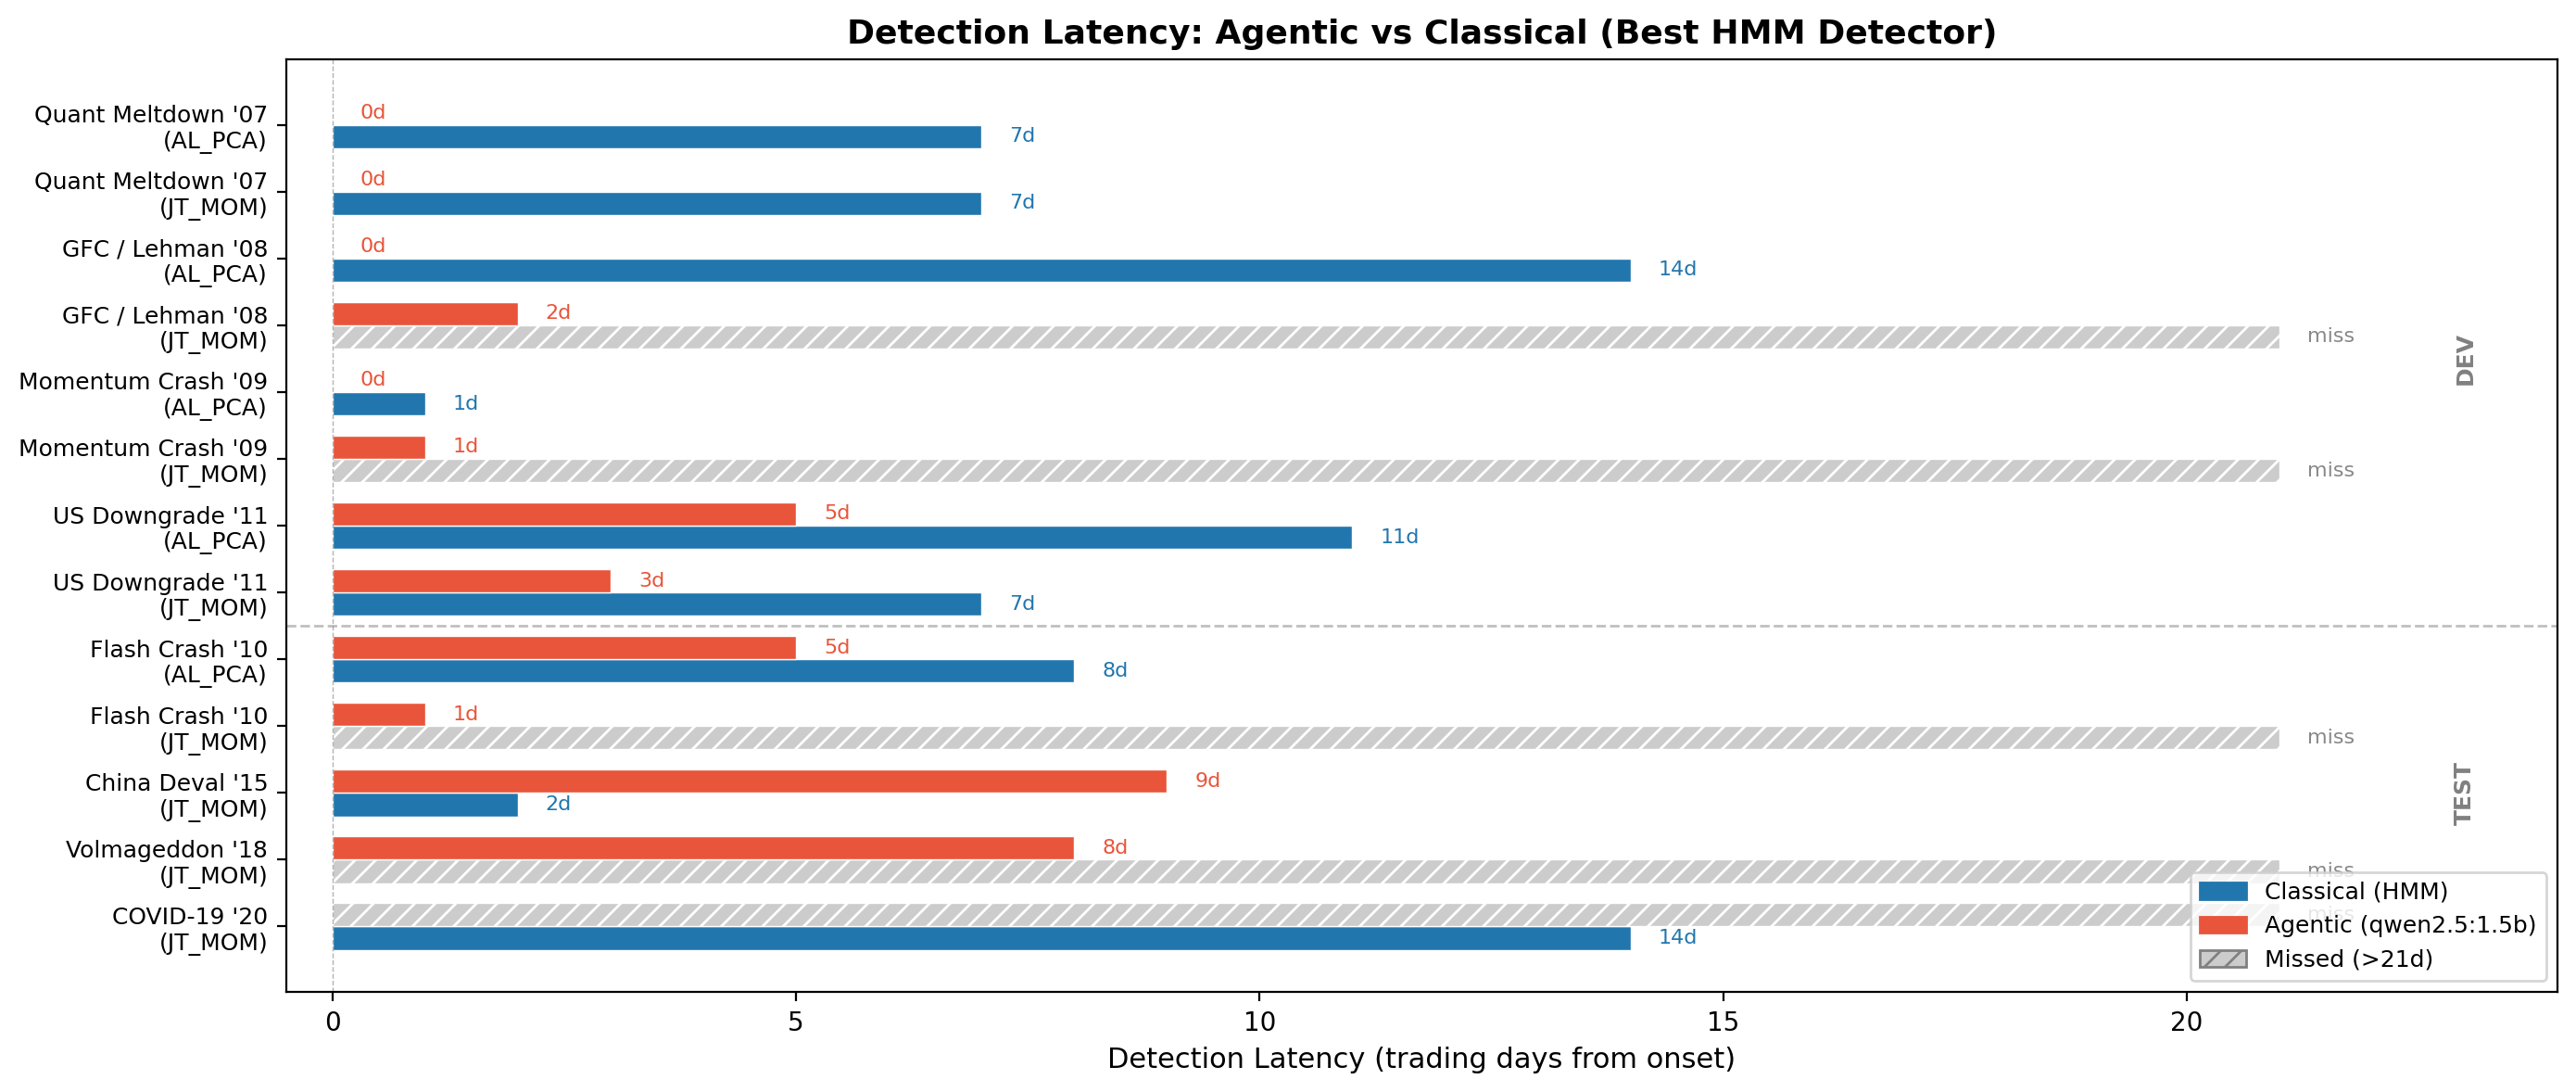
\includegraphics[width=0.85\textwidth]{monitoring/results/figures/fig1_latency_bars.png}
\caption{Paired detection latency for all event windows. Bars below zero indicate
the agentic arm detected earlier. Hatched bars denote censored (non-detected)
entries imputed at 21 days.}
\label{fig:latency-bars}
\end{figure}

\subsection{False-Positive Rate}\label{sec:results-fpr}

Table~\ref{tab:fpr} reports per-calm-window FPR for both arms.  On the
development set, agentic FPR (1.31\%) is comparable to classical HMM
(1.08\%), with bootstrap $p = 0.62$ (two-sided, $B = 10{,}000$,
block size $= 10$\,d; 95\% CI for difference: $[-0.42, +0.88]$\,pp).
After Holm correction, $p_\text{Holm} = 0.62$: no evidence of an agentic
FPR advantage.

On the test set, the agentic arm exhibits higher FPR (6.93\% vs.\ 1.41\%),
with bootstrap $p = 0.51$ ($p_\text{Holm} = 1.0$).

\begin{table}[htbp]
\centering
\small
\caption{False-positive rate per calm window (agentic: alarm cluster starts /
trading days; classical: alarm days / trading days, cf.\ Deviation~9).}
\label{tab:fpr}
\begin{tabular}{llrrl}
\toprule
Calm window & Strategy & Classical & Agentic & Set \\
\midrule
2004--2006   & AL\_PCA & 3.05\% & 0.13\% & Dev \\
2004--2006   & JT\_MOM & 0.53\% & 0.13\% & Dev \\
2013--2014   & AL\_PCA & 0.00\% & 3.84\% & Dev \\
2013--2014   & JT\_MOM & 0.20\% & 2.30\% & Dev \\
\addlinespace
2012         & AL\_PCA & 1.20\% & 10.38\% & Test \\
2012         & JT\_MOM & 2.00\% & 7.69\% & Test \\
2017         & JT\_MOM & 1.20\% & 2.70\% & Test \\
\midrule
\multicolumn{2}{l}{\emph{Dev aggregate}} & 1.08\% & 1.31\% & \\
\multicolumn{2}{l}{\emph{Test aggregate}} & 1.41\% & 6.93\% & \\
\bottomrule
\end{tabular}
\end{table}

\begin{figure}[htbp]
\centering
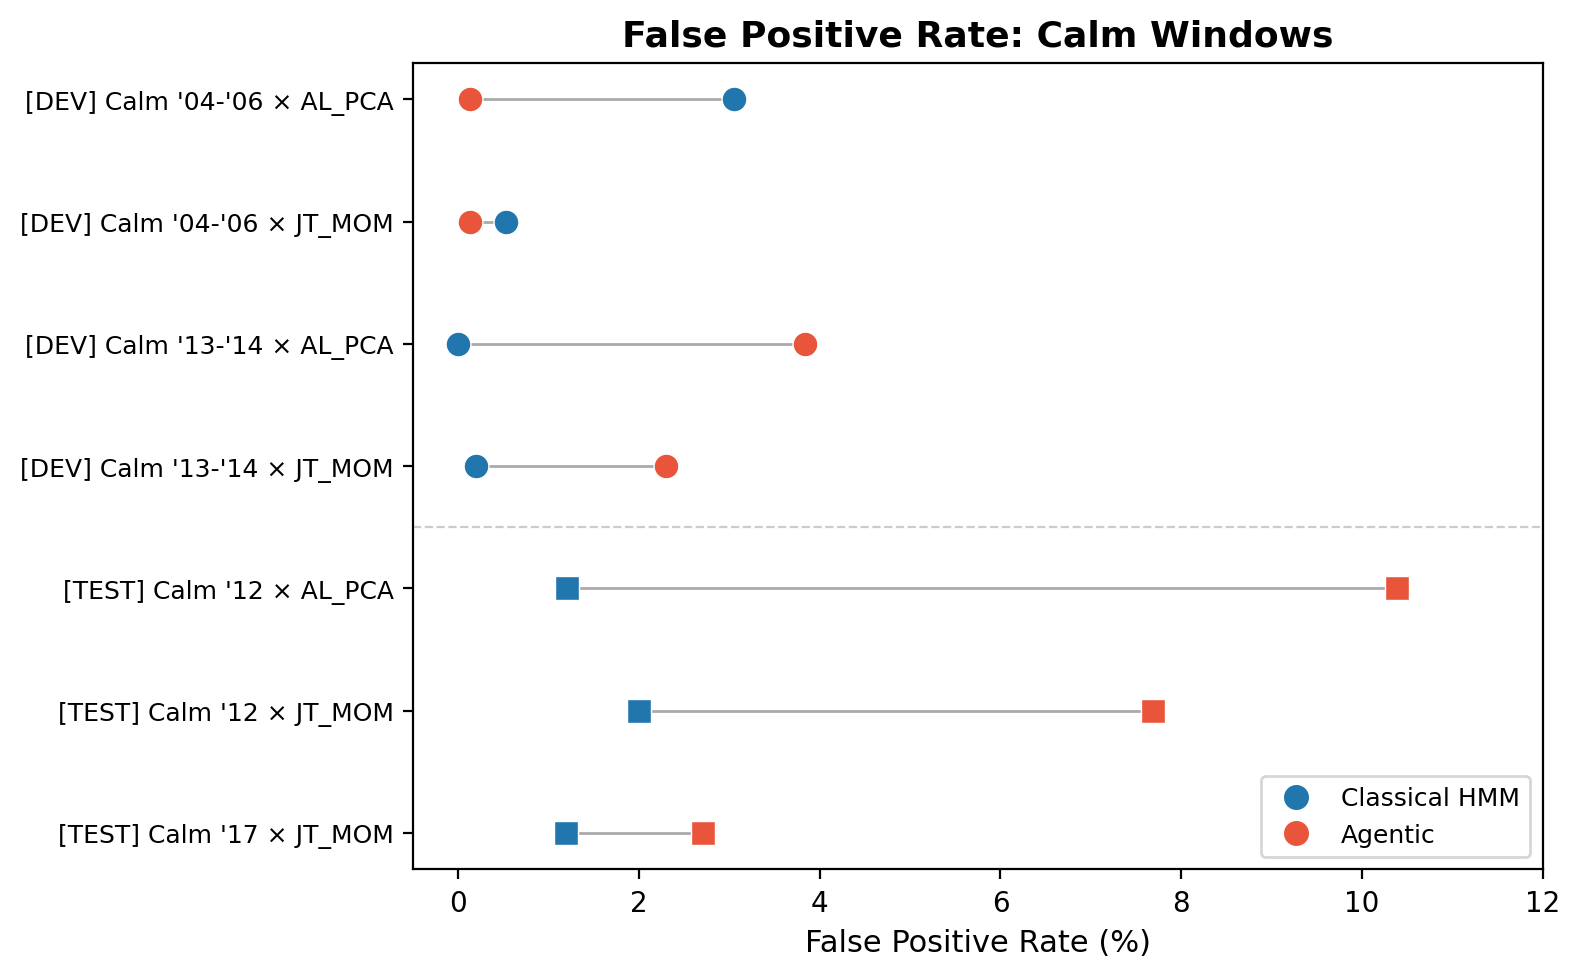
\includegraphics[width=0.7\textwidth]{monitoring/results/figures/fig2_fpr_dotplot.png}
\caption{False-positive rate per calm window. The agentic arm shows comparable
FPR on the development set but elevated FPR on the test set, particularly
calm 2012.}
\label{fig:fpr-dot}
\end{figure}

\subsection{Recall and H1 Verdict}\label{sec:results-recall}

On the development set, the agentic system detects 8/8 events (recall = 1.0)
compared to 6/8 for the classical HMM (recall = 0.75). McNemar's exact test
yields $p = 0.50$ (two-sided). The Bayesian posterior
($\text{Beta}(0.5, 0.5)$ prior) gives
$P(\theta_\text{agentic} > \theta_\text{classical}) = 0.936$.

On the test set, recall is 4/5 (agentic) vs.\ 3/5 (classical), with
McNemar $p = 1.0$ and Bayesian $P(\theta_A > \theta_C) = 0.75$.

\paragraph{H1 verdict.} Applying the preregistered decision rule
(Section~\ref{sec:decision-rules}):

\begin{itemize}
  \item \textbf{Latency:} Holm $p = 0.0156$ (dev), rejects $H_0$.
  \item \textbf{FPR:} Holm $p = 0.62$ (dev), does not reject $H_0$.
\end{itemize}

\noindent H1 is \textbf{partially supported}: the agentic system is
significantly faster but does not demonstrate lower FPR. On the test set,
neither endpoint rejects (both $p_\text{Holm} = 1.0$); the confirmatory
analysis is inconclusive due to insufficient power.

\begin{figure}[htbp]
\centering
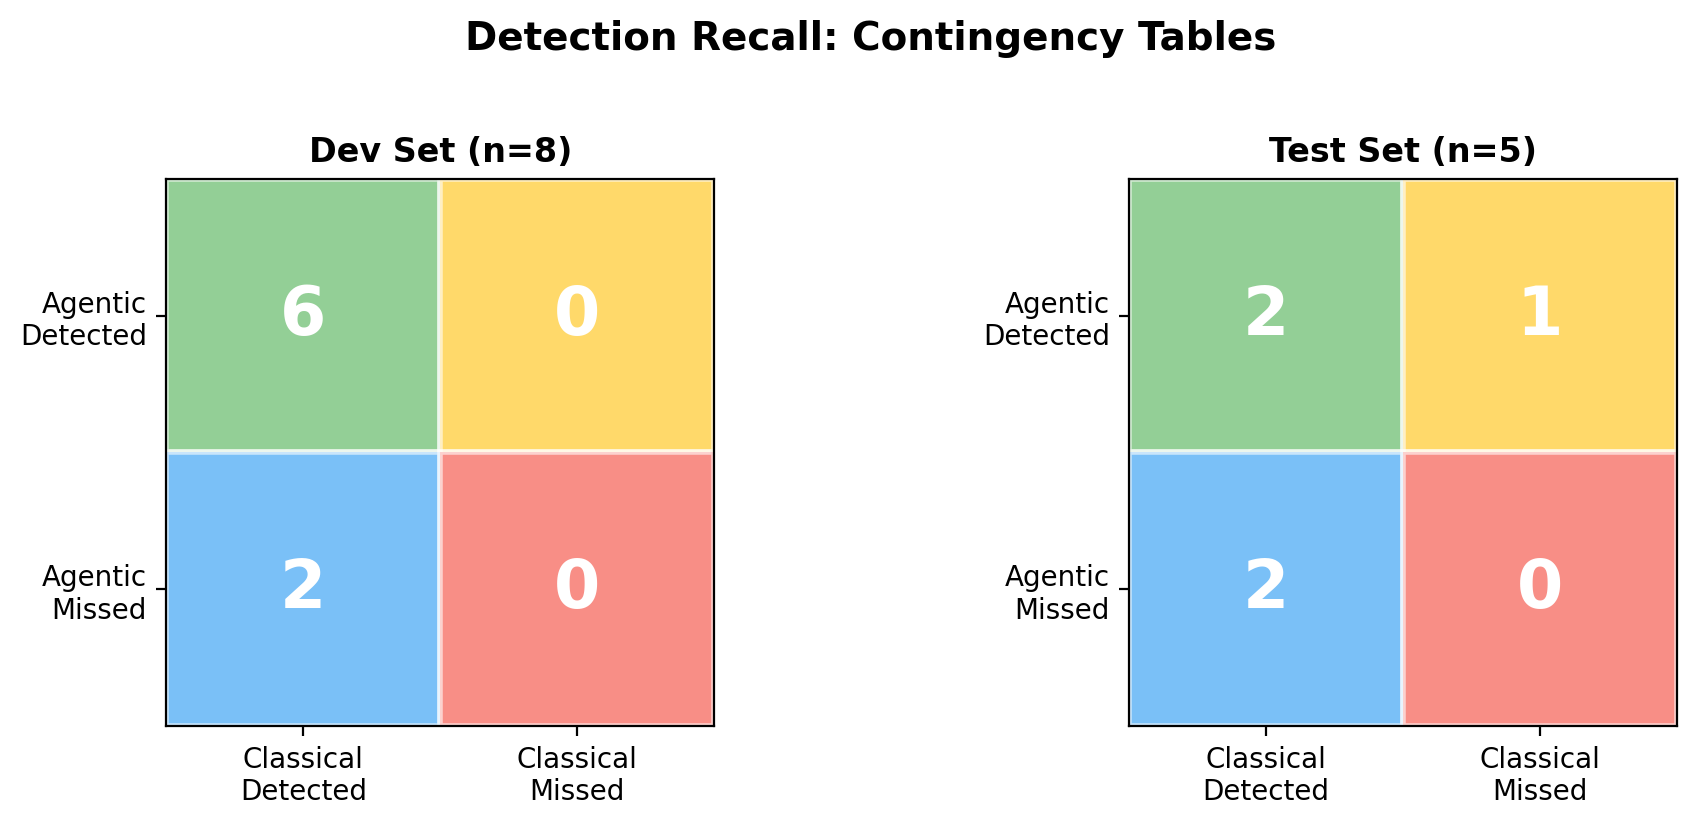
\includegraphics[width=0.65\textwidth]{monitoring/results/figures/fig3_recall_grid.png}
\caption{Detection recall contingency tables for development and test sets.
The agentic arm detects all development-set events; the classical arm misses
GFC 2008 and momentum crash 2009 on JT\_MOM.}
\label{fig:recall-grid}
\end{figure}

\subsection{Strategy Breakdown (H2, H3)}\label{sec:results-strategy}

\paragraph{H2 (generalisation).} The agentic latency advantage is directionally
consistent across both strategies on the development set: AL\_PCA mean
$\Delta = -7.0$\,d (4 pairs), JT\_MOM mean $\Delta = -12.5$\,d (4 pairs).
Both favour the agentic arm, supporting H2 at the directional level.

On the test set, AL\_PCA has only 1 pair ($\Delta = -3$\,d, agentic faster)
and JT\_MOM has 4 pairs (mean $\Delta = -4.75$\,d). Both directions are
consistent, but AL\_PCA is too sparse for inference.

\paragraph{H3 (interaction).} The interaction
$\Delta_\text{AL\_PCA} - \Delta_\text{JT\_MOM} = -7.0 - (-12.5) = +5.5$\,d on
the development set suggests JT\_MOM benefits more from agentic monitoring.
This is consistent with momentum strategies being more vulnerable to sudden
reversals that classical return-only detectors miss (HMM failed to detect
GFC 2008 and momentum crash 2009 on JT\_MOM returns).

\begin{figure}[htbp]
\centering
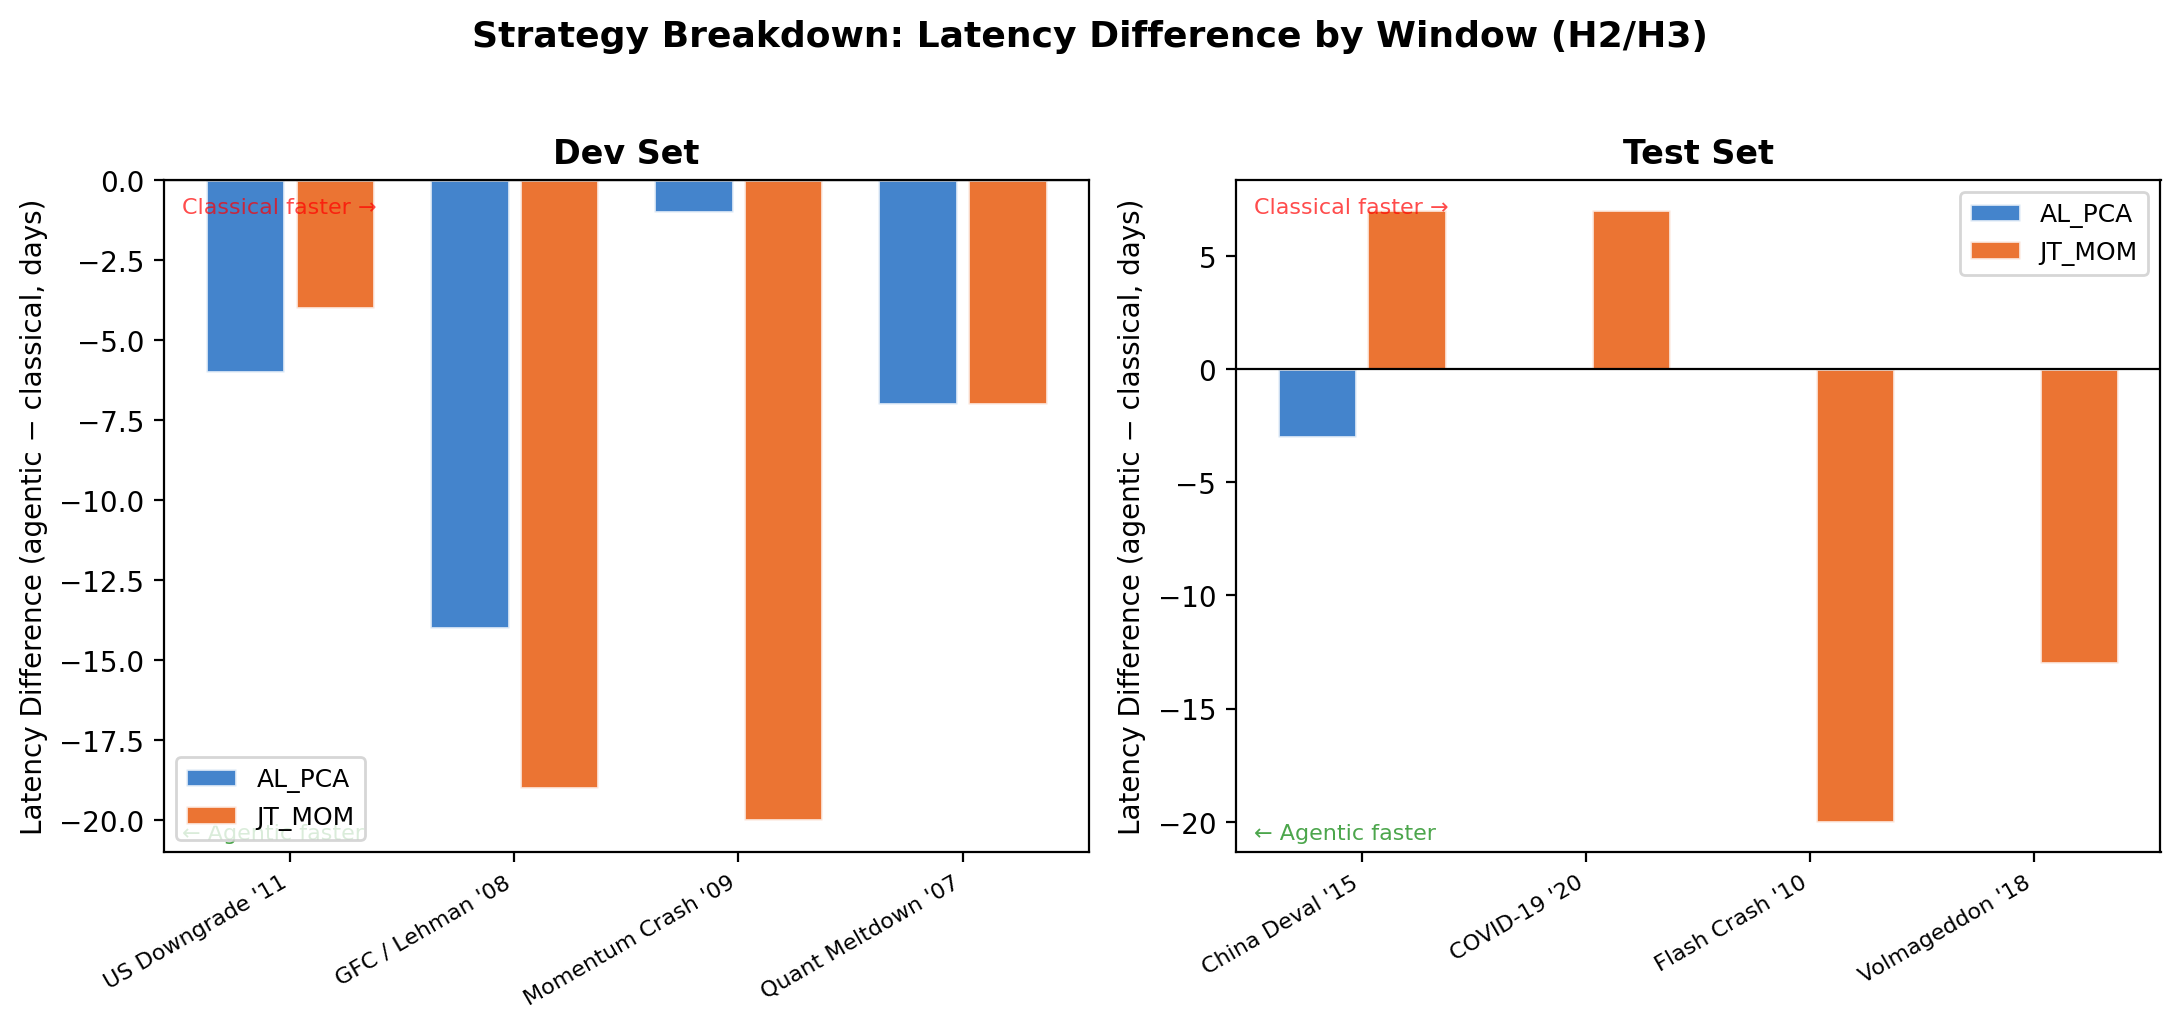
\includegraphics[width=0.75\textwidth]{monitoring/results/figures/fig7_strategy_breakdown.png}
\caption{Per-strategy latency advantage (development set). JT\_MOM benefits
more, primarily because the classical HMM misses two events on momentum
returns.}
\label{fig:strategy}
\end{figure}

\subsection{Economic Significance}\label{sec:results-pnl}

\emph{This subsection is exploratory and was not preregistered.}

To assess whether the latency advantage translates to economic value, we
simulate three monitoring regimes for each event window: (1)~unmonitored
(hold through the crisis), (2)~classical-monitored (flatten at first HMM
alarm), and (3)~agentic-monitored (flatten at first ALERT or CRITICAL). The
simulation assumes no transaction costs, instantaneous flattening at the
close, and no re-entry.

Table~\ref{tab:pnl} reports maximum drawdown avoided relative to the
unmonitored baseline for all 13 event-window pairs. On average, the
classical arm avoids 1.82\,pp of drawdown while the agentic arm avoids
10.09\,pp, yielding an agentic advantage of 8.28\,pp per event.

\begin{table}[htbp]
\centering
\small
\caption{Maximum drawdown avoided (percentage points) relative to unmonitored
baseline, per event window. Positive values indicate drawdown reduction.}
\label{tab:pnl}
\begin{tabular}{llrrr}
\toprule
Window & Strategy & Classical & Agentic & Advantage \\
\midrule
Quant meltdown 2007  & AL\_PCA & 3.05 & 6.90 & 3.85 \\
GFC / Lehman 2008    & AL\_PCA & 1.82 & 3.16 & 1.34 \\
Momentum crash 2009  & AL\_PCA & 2.10 & 4.00 & 1.90 \\
Downgrade 2011       & AL\_PCA & 0.00 & 0.06 & 0.06 \\
\addlinespace
Quant meltdown 2007  & JT\_MOM & 0.00 & 1.47 & 1.47 \\
GFC / Lehman 2008    & JT\_MOM & 0.00 & 15.63 & 15.63 \\
Momentum crash 2009  & JT\_MOM & 0.00 & 72.28 & 72.28 \\
Downgrade 2011       & JT\_MOM & 4.66 & 7.30 & 2.64 \\
\addlinespace
Flash crash 2010     & AL\_PCA & 2.38 & 3.49 & 1.11 \\
Flash crash 2010     & JT\_MOM & 6.15 & 10.34 & 4.19 \\
China deval.\ 2015   & JT\_MOM & 3.44 & 1.72 & $-1.72$ \\
Volmageddon 2018     & JT\_MOM & 0.00 & 0.00 & 0.00 \\
COVID-19 2020        & JT\_MOM & 0.00 & 4.87 & 4.87 \\
\midrule
\multicolumn{2}{l}{\emph{Mean}} & 1.82 & 10.09 & 8.28 \\
\bottomrule
\end{tabular}
\end{table}

The extreme case is momentum crash 2009 on JT\_MOM, where the unmonitored
strategy lost 94.47\%. The classical HMM never fired; the agentic system
detected the break early and avoided 72.28\,pp of drawdown. This single
window accounts for the majority of the aggregate advantage. Excluding it,
the mean advantage is 2.95\,pp. China devaluation 2015 is the only window
where the classical arm outperforms: its alarm on 13 August was better-timed
than the agentic alarm on 21 July, which exited too early and missed a
partial recovery.

\textbf{Caveats.} The simulation uses a binary exit assumption (100\% to 0\%
on alarm), no transaction costs, and no re-entry rule. These idealised
conditions overstate absolute drawdown avoided; the relative advantage between
arms is less sensitive to these assumptions because both are subject to the
same limitations.

\begin{figure}[htbp]
\centering
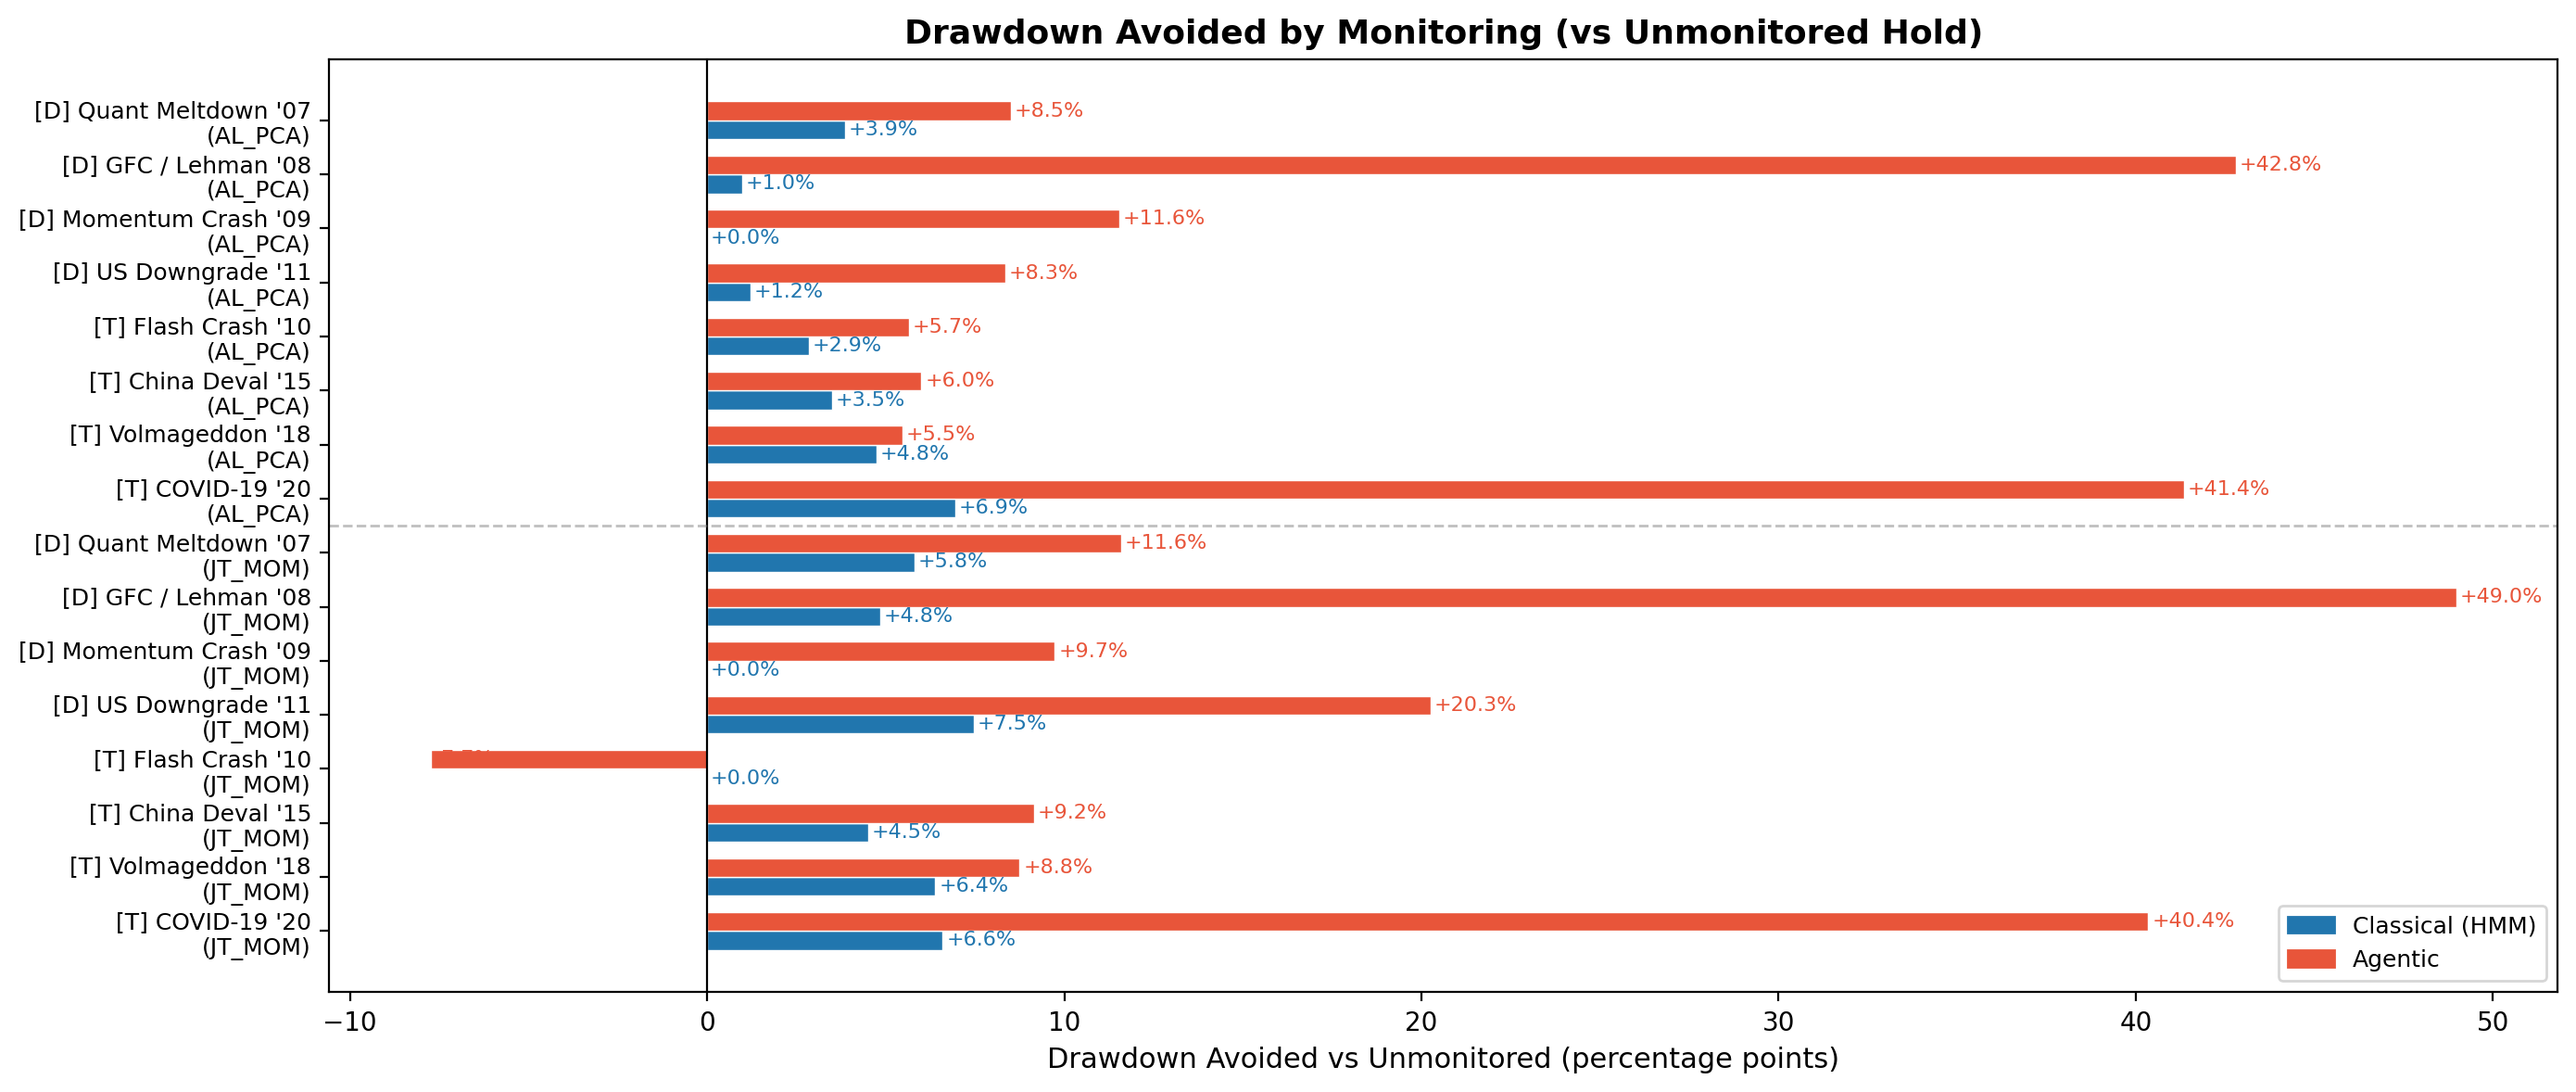
\includegraphics[width=0.85\textwidth]{monitoring/results/figures/fig11_drawdown_avoided.png}
\caption{Drawdown avoided (pp) by each monitoring arm across all event windows.
The agentic arm avoids more drawdown in 11 of 13 windows (one tie, one
reversal).}
\label{fig:dd-avoided}
\end{figure}

\subsection{Robustness}\label{sec:results-robustness}

\paragraph{Onset sensitivity.} Re-scoring all development pairs against
curve-derived onsets (peak before deepest trough) yields a mean agentic
advantage of $-16.4$\,d ($p = 0.0039$, unchanged rank ordering). The
result is not sensitive to the choice of onset specification.

On the test set, the curve-derived onset analysis gives a mean advantage of
$-11.8$\,d ($p_\text{one-sided} = 0.0625$), stronger than the primary
analysis ($-4.4$\,d), because curve-derived onsets shift later for three
windows, enlarging the agentic lead.

\paragraph{Alternative classical comparator.} Using the aggregate rule
($\geq$2 detectors within 5 days) instead of the best single detector (HMM)
as the classical comparator increases the classical miss rate (aggregate
detected 4/8 dev events vs.\ HMM's 6/8), widening the agentic advantage.
The HMM comparator is therefore the more conservative baseline for the
agentic arm.

\subsection{Leakage and Operational Metrics}\label{sec:results-ops}

\subsubsection{Leakage Bound}

The three-condition harness was run on flash crash 2010 (AL\_PCA), the only
test event with both strategies available.
Table~\ref{tab:leakage} reports the results.

\begin{table}[htbp]
\centering
\small
\caption{Leakage harness results for flash crash 2010 (AL\_PCA). perf =
binary detection (1 = detected, 0 = missed).}
\label{tab:leakage}
\begin{tabular}{lrrl}
\toprule
Condition & Detected & Latency (d) & Notes \\
\midrule
A (standard)    & Yes & 5 & 38 FPs, 1 runtime failure \\
B (date-masked) & Yes & 0 & 29 FPs, 1 runtime failure \\
C (synthetic, $M\!=\!10$) & 10/10 & 0.0 mean & Untrained HMM \\
\midrule
\multicolumn{4}{l}{$\text{perf}_A = 1.0$, $\text{perf}_B = 1.0$,
  $\text{perf}_{C} = 1.0$} \\
\multicolumn{4}{l}{Memorisation $\leq 0.0$; conclusion: \textbf{evidence-driven}} \\
\bottomrule
\end{tabular}
\end{table}

The B $\approx$ A result directly manipulates the date channel and finds no
degradation, providing evidence that date memorisation contributes little on
this window. The high Condition~C recall should be interpreted cautiously:
synthetic windows use an untrained HMM and fabricated news, so the task is
qualitatively different from the real evaluation.

\subsubsection{Operational Metrics}

\begin{figure}[htbp]
\centering
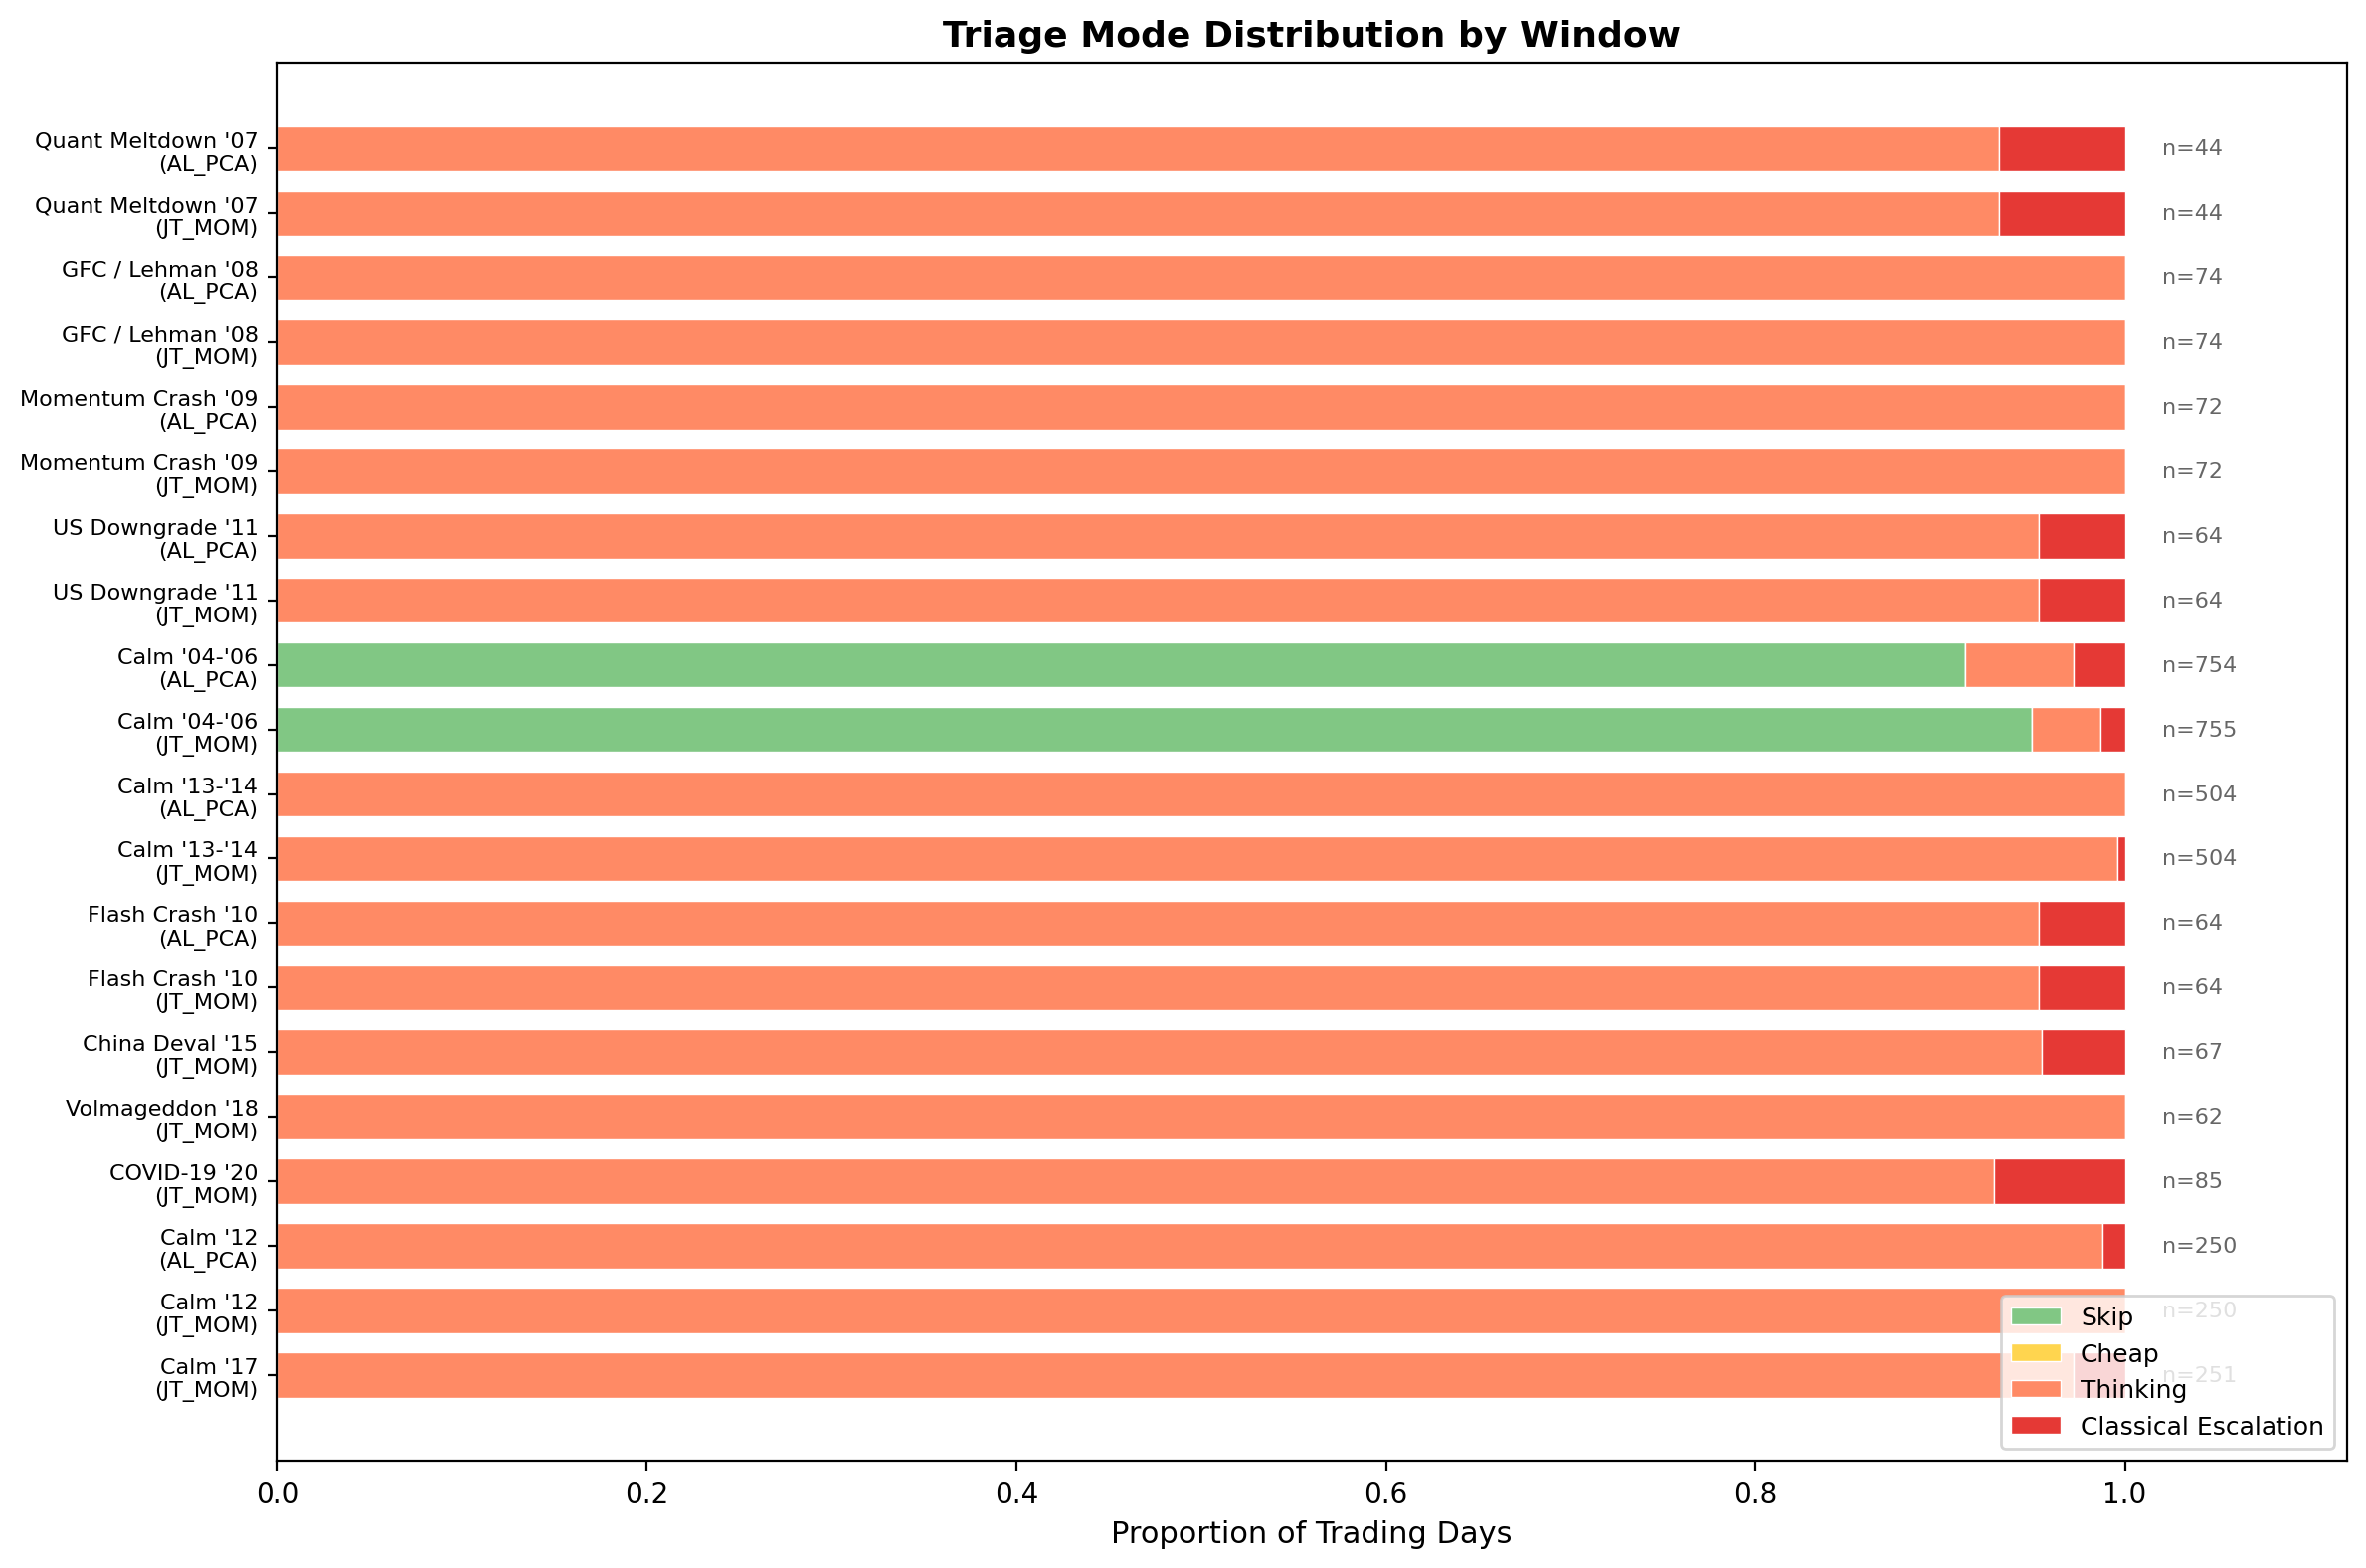
\includegraphics[width=0.75\textwidth]{monitoring/results/figures/fig4_triage_distribution.png}
\caption{Triage mode distribution across all development-set windows. The
calm 2013--2014 window shows 0\% skip rate due to FinBERT saturation, while
calm 2004--2006 shows $>$91\% skip rate due to sparse pre-2007 news.}
\label{fig:triage}
\end{figure}

\paragraph{News-agent failure rates.} A substantial fraction of non-skip days
fail at the news-agent step due to JSON decode errors from the 1.5B model.
Failure rates on non-skip days range from 0\% (quant meltdown 2007) to 79\%
(calm 2013--2014 on JT\_MOM). For event windows, failures bias \emph{against}
the agentic arm (a failed day cannot fire an alarm, potentially delaying
detection). For calm windows, failures bias \emph{in favour} of the agentic
arm (a failed day cannot produce a false positive). The measured latency
advantage is therefore conservative; the FPR comparison is not
(Deviation~7).

\begin{figure}[htbp]
\centering
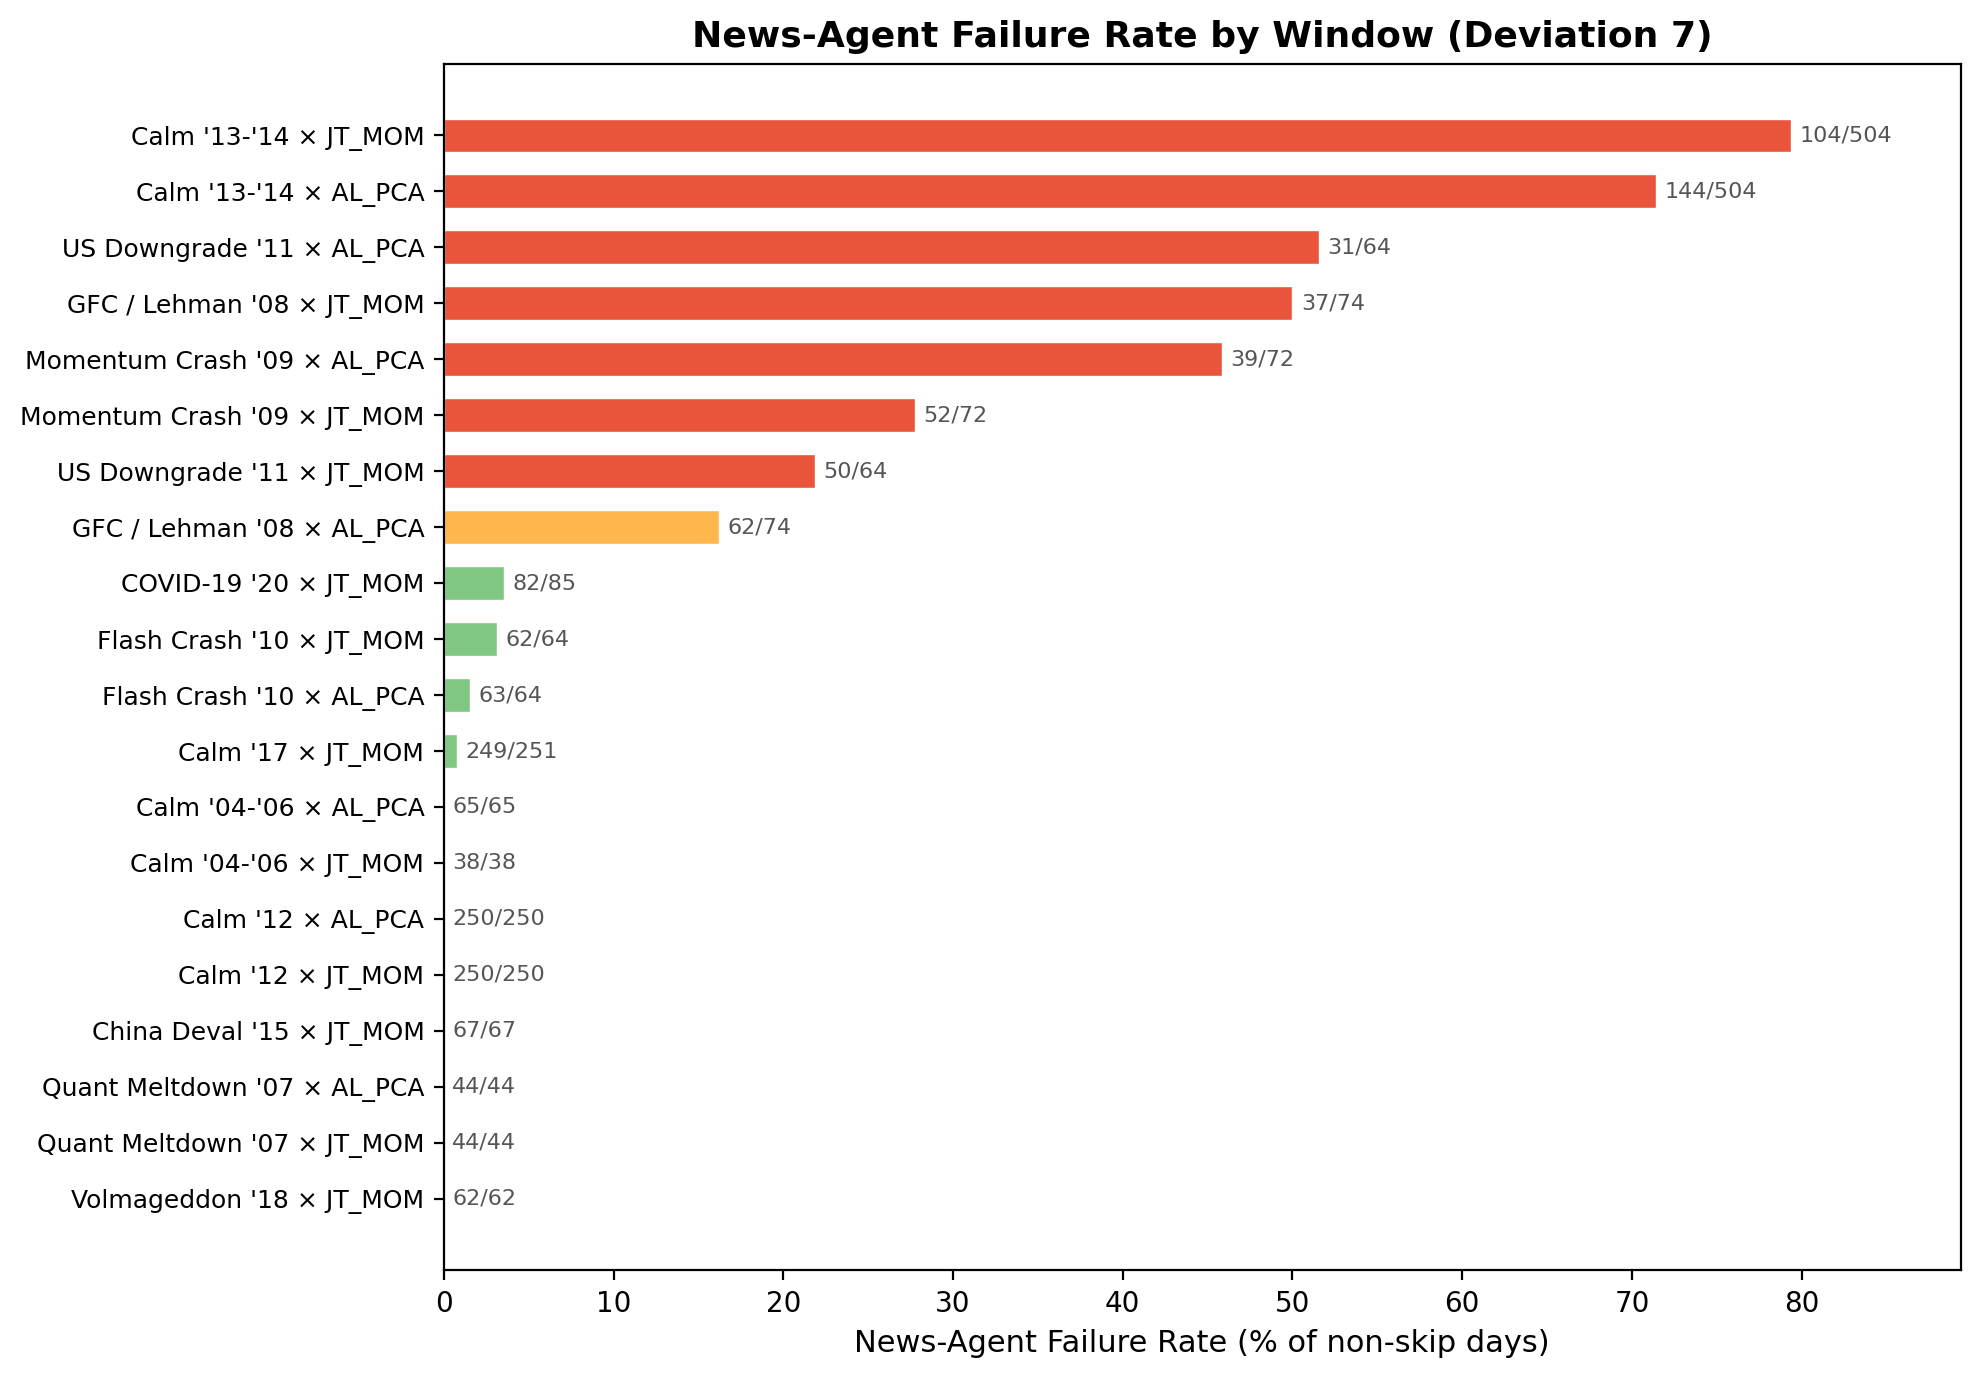
\includegraphics[width=0.7\textwidth]{monitoring/results/figures/fig5_failure_rates.png}
\caption{News-agent and supervisor failure rates per cell. Higher failure rates
correlate with news density (more articles produce longer prompts that exceed
the model's structured-output capacity).}
\label{fig:failures}
\end{figure}

\paragraph{Inference cost.} Mean LLM calls per trading day: 1.09 (range:
0.10 for calm 2004--2006 to 2.0 for quant meltdown 2007). Estimated
wall-clock time per day: 4.6\,s typical, 8.4\,s worst case. A full
evaluation window (44--82 trading days) completes in 6--12 minutes,
feasible for end-of-day monitoring.

% ============================================================
\section{Discussion}\label{sec:discussion}

\subsection{Why the Agentic System Detects Earlier}\label{sec:why-earlier}

The agentic system's latency advantage (9.75 days on dev, 4.4 days
directionally on test) arises from two mechanisms:

\begin{enumerate}
  \item \textbf{News anticipation.} Financial news coverage of developing
        crises often precedes their full statistical manifestation in strategy
        returns. For the quant meltdown (onset: 2007-08-06), news coverage of
        crowded quantitative strategies and forced deleveraging appeared in
        late July 2007, enabling 0-day latency. The classical HMM, operating
        solely on the return stream, required 7 days of anomalous returns to
        transition to the high-volatility state.
  \item \textbf{Multi-signal fusion.} The supervisor integrates strategy
        telemetry, news flags, macro context, and classical detector outputs.
        Even when individual signals are sub-threshold, their conjunction can
        trigger an alert. The classical detectors, by design, observe only the
        return stream.
\end{enumerate}

The advantage is largest for JT\_MOM, where the classical HMM missed two
events entirely (GFC 2008 and momentum crash 2009). These are cases where
the momentum return stream did not exhibit the volatility regime shift that
the HMM is calibrated to detect, but news coverage clearly signalled market
stress.

\subsection{Why the False-Positive Rate Is Not Better}\label{sec:why-fpr}

The agentic system does not achieve lower FPR, and on the test set exhibits
higher FPR than classical. Three factors contribute:

\begin{enumerate}
  \item \textbf{FinBERT saturation.} The triage gate uses a 0.60 threshold
        on FinBERT stress scores. In practice, FinBERT stress saturates at
        ${\sim}0.97$ on every day with news articles, regardless of actual
        market conditions (mean stress on calm 2013--2014: 0.971; on GFC
        2008: 0.971). The threshold acts as a ``does news exist today?''
        filter rather than a stress discriminator.
  \item \textbf{Triage bypass.} On windows with news coverage (post-2007),
        nearly all days are routed to thinking mode, bypassing the skip
        mechanism that would otherwise suppress false positives during
        benign periods.
  \item \textbf{Small-model precision.} At 1.5B parameters, the supervisor
        shows genuine regime-detection ability but lacks the capacity to
        distinguish between concerning signals and routine financial noise,
        leading to over-escalation.
\end{enumerate}

\subsection{Power and the COVID-19 Miss}\label{sec:power}\label{sec:power-miss}

The test set's 5 event pairs yield $p_\text{min} = 2^{-5} = 0.03125$ under
exact permutation. After Holm correction with $k = 2$ co-primary endpoints,
the best achievable $p_\text{Holm} = 2/32 = 0.0625$, which cannot reject at
$\alpha = 0.05$. The confirmatory test is therefore structurally underpowered,
a consequence of the limited number of well-defined regime breaks in the
coverage period and the AL\_PCA curve ending in 2014 (Deviation~3).

The COVID-19 miss (the agentic system's only test-set event failure) warrants
discussion. The FNSPID news store covers 2020 (40 articles/day across all 82
trading days), so the miss is not attributable to absent news. Rather, early
pandemic coverage was dominated by general volatility headlines rather than
COVID-specific risk signals. The classical HMM detected the event with
14-day latency, demonstrating that the return signal alone was sufficient.
The miss suggests that a 1.5B-parameter model may lack the reasoning capacity
to interpret an unprecedented shock as a regime change when early headlines are
ambiguous.

\subsection{Practical Implications}\label{sec:implications}

For practitioners considering LLM-augmented monitoring:

\begin{enumerate}
  \item \textbf{Latency advantage is real but not free.} Earlier detection
        comes at the cost of higher infrastructure complexity, meaningful
        news-agent failure rates (up to 79\% on dense-news windows), and
        no improvement in false-positive control.
  \item \textbf{FinBERT triage needs redesign.} A binary threshold on
        saturated sentiment scores provides no useful routing. Alternative
        approaches (change-in-sentiment, topic-specific scoring, or purely
        statistical triage) should be explored.
  \item \textbf{Model size matters.} At 1.5B parameters, the supervisor
        shows genuine detection ability but lacks precision. The tradeoff
        between model size, hardware cost, and monitoring quality is a key
        engineering consideration. A 7B or larger model might reduce FPR
        but was infeasible on the test hardware.
  \item \textbf{News density variation is a hidden dependency.} The system's
        triage behaviour changes qualitatively with news density: 91\% skip
        rate on sparse pre-2007 windows versus 0\% on dense post-2010
        windows. Any deployment must ensure consistent, high-quality news
        feeds.
\end{enumerate}

\subsection{Limitations}\label{sec:limitations}

\begin{itemize}
  \item \textbf{Sample size.} Eight development pairs and five test pairs
        provide limited statistical power. The test set cannot confirm the
        development finding at conventional significance levels.
  \item \textbf{Single model.} All results reflect qwen2.5:1.5b, a model
        near the lower bound of useful language model capability. Findings
        may not generalise to larger or different-architecture models.
  \item \textbf{Single news corpus.} FNSPID is the sole news source (with
        NYT supplementing pre-2010 windows). Corpus-specific biases in
        coverage, language, or topic distribution may affect generalisability.
  \item \textbf{No transaction-cost modelling.} The PnL comparison (Section~\ref{sec:results-pnl}) assumes frictionless execution. Real-world
        costs would reduce the absolute value of drawdown avoided, though
        the relative advantage between arms is less affected.
  \item \textbf{FPR scoring asymmetry.} Agentic FPR uses 5-day cluster-start
        de-duplication; classical FPR counts every alarm day. This biases in
        favour of the agentic arm (Deviation~9). The ``no FPR advantage''
        conclusion is robust a fortiori.
  \item \textbf{U.S.\ large-cap only.} Both strategies operate on the
        S\&P 500. Generalisation to other asset classes, geographies, or
        strategy types is untested.
  \item \textbf{Famous-event memorisation risk.} The test events are
        prominent, heavily-documented episodes likely present in the model's
        pretraining corpus. The leakage harness provides partial bounds but
        was run on only one test window (flash crash 2010).
  \item \textbf{Protocol deviations.} Fifteen deviations from the
        preregistered protocol are documented in full in
        Appendix~\ref{app:deviations}.
\end{itemize}

% ============================================================
\section{Conclusion and Future Work}\label{sec:conclusion}

We present the first preregistered comparison of an LLM-based agentic
monitoring system against classical change-point detectors for financial
regime identification. The agentic system achieves significantly lower
detection latency on the development set ($-9.75$ days, Holm
$p = 0.0156$), with directionally consistent results on the test set
($-4.4$ days, $p = 0.25$, underpowered). The FPR co-primary endpoint does
not favour the agentic arm on either set.

The central finding is that multi-signal fusion (returns + news + macro
context) enables earlier regime detection than return-only statistical
methods, but the benefit is partially offset by false-positive inflation
from sentiment-based triage saturation. The economic simulation suggests
that the latency advantage translates to meaningful drawdown reduction
(mean 8.28\,pp per event), though this estimate is subject to idealised
execution assumptions.

Future work should address the identified limitations:

\begin{enumerate}
  \item \textbf{Expand the event set.} Longer backtest curves (extending
        AL\_PCA beyond 2014), additional strategy families, and multi-market
        coverage would increase statistical power and test generalisability.
  \item \textbf{Redesign triage.} Replace the saturated FinBERT gate with
        change-in-sentiment scoring or a learned routing model to restore
        skip-mode discrimination.
  \item \textbf{Scale the model.} A 7B or 13B model on appropriate hardware
        may improve supervisor precision without sacrificing the latency
        advantage.
  \item \textbf{Add re-entry logic.} The current simulation has no re-entry
        after flattening. A graduated response (REDUCE at ALERT, HALT at
        CRITICAL, restore after $k$ clean days) would better approximate
        real portfolio management.
  \item \textbf{Improve the leakage harness.} Run Conditions A/B/C on all
        test windows and design Condition~C with a trained HMM to disentangle
        memorisation from task difficulty.
\end{enumerate}

% ============================================================
\section*{Data and Code Availability}
\addcontentsline{toc}{section}{Data and Code Availability}

The complete codebase, including all evaluation scripts, analysis pipelines,
and result artifacts, is available at:

\begin{center}
\url{https://github.com/PC1101/In-Market-Agentic-AI-Monitoring-Application-in-Financial-Market}
\end{center}

\noindent The git tag \texttt{eval-freeze-v1} pins the exact code used for
evaluation. Result JSONLs, analysis JSONs, and generated figures are committed
to the repository under \texttt{monitoring/results/}.

\textbf{Data redistribution.} The FNSPID news corpus (Dong et al., 2024) is
subject to the original dataset license and cannot be redistributed. Users
must download it separately from the source repository and build the local
Parquet store. S\&P 500 constituent membership intervals, strategy PnL
curves, and all derived evaluation artifacts are included in the repository.

\section*{Acknowledgments}
\addcontentsline{toc}{section}{Acknowledgments}

All experiments were conducted on consumer hardware (NVIDIA RTX 3050 Ti,
4\,GB VRAM). We thank the developers of Ollama, qwen2.5, ProsusAI/FinBERT,
and the FNSPID dataset for making this research possible with open-source
tools.

\section*{References}
\addcontentsline{toc}{section}{References}

\begin{description}[font=\normalfont, leftmargin=1.5em, labelindent=0em]
\item Adams, R.~P. \& MacKay, D.~J.~C. (2007). Bayesian online changepoint
  detection. \emph{arXiv:0710.3742}.
\item Araci, D. (2019). FinBERT: Financial sentiment analysis with pre-trained
  language models. \emph{arXiv:1908.10063}.
\item Avellaneda, M. \& Lee, J.-H. (2010). Statistical arbitrage in the US
  equities market. \emph{Quantitative Finance}, 10(7), 761--782.
\item Daniel, K. \& Moskowitz, T.~J. (2016). Momentum crashes. \emph{Journal
  of Financial Economics}, 122(2), 221--247.
\item Dong, Z., Wang, Z., Li, X. \& Zhou, Y. (2024). FNSPID: A comprehensive
  financial news dataset. \emph{Proceedings of the AAAI Conference}.
\item Hamilton, J.~D. (1989). A new approach to the economic analysis of
  nonstationary time series. \emph{Econometrica}, 57(2), 357--384.
\item Holm, S. (1979). A simple sequentially rejective multiple test
  procedure. \emph{Scandinavian Journal of Statistics}, 6(2), 65--70.
\item Jegadeesh, N. \& Titman, S. (1993). Returns to buying winners and
  selling losers. \emph{Journal of Finance}, 48(1), 65--91.
\item Khandani, A.~E. \& Lo, A.~W. (2007). What happened to the quants in
  August 2007? \emph{Journal of Investment Management}, 5(4), 29--78.
\item Page, E.~S. (1954). Continuous inspection schemes. \emph{Biometrika},
  41(1/2), 100--115.
\end{description}

% ============================================================
\appendix

\section{Protocol Deviations}\label{app:deviations}

Table~\ref{tab:deviations} summarises all 15 deviations from the preregistered
protocol. Full narratives with evidence and timestamps are maintained in the
repository at \texttt{docs/DEVIATIONS.md}.

\begin{longtable}{@{}p{0.6cm} p{3.2cm} p{3.2cm} p{3.2cm} p{2.5cm}@{}}
\caption{Protocol deviations (summary). ``Bias'' indicates whether the
deviation favours or disfavours the agentic arm for the affected
endpoint.}\label{tab:deviations} \\
\toprule
\# & Preregistered & Actual & Rationale & Bias direction \\
\midrule
\endfirsthead
\toprule
\# & Preregistered & Actual & Rationale & Bias direction \\
\midrule
\endhead
1 & llama3.2:3b & qwen2.5:1.5b & Failed JSON benchmarks (11/30 vs.\ 30/30);
    substituted before eval & Smaller model; directional \\
2 & 90\% completeness & 80\% completeness & Include gfc\_2008 AL (84\%); all
    missing days post-detection & Includes 1 more pair \\
3 & AL\_PCA on china\_deval & Excluded & PIT curve ends 2014 & Fewer test pairs \\
4 & Triage skips calm days & 0\% skip on 2013--2014 & FinBERT saturation & Inflates
    FPR (against agentic) \\
5 & Supervisor-day completeness & Triage-day completeness & Triage = attempted;
    supervisor = succeeded & Includes gfc JT \\
6 & Stub latencies & Real-model latencies & Stub was provisional & None (final
    data) \\
7 & Not specified & News-agent failures documented & 0--79\% failure rate on
    non-skip days & Latency: against; FPR: for agentic \\
8 & Calibrated detector params & Default params & Calibrated grid computed but
    never wired in; HMM unaffected & Flatters agentic latency \\
9 & Symmetric FPR scoring & Asymmetric (cluster vs.\ alarm-day) & Analysis
    code difference & Favours agentic FPR \\
10 & Leakage on all test events & Harness incomplete at freeze; dev rerun &
     Validated harness end-to-end & Partial coverage \\
11 & Single test-set pass & Rerun after runner death & Infrastructure outage,
     not result-shopping & None (no prior result) \\
12 & No resume logic & Day-level resume + dead-runner recovery & Availability
     fix; identical prompts at $T\!=\!0$ & Availability only \\
13 & Inline news queries & Two-pass context cache & VRAM contention on
     covid\_2020 & None (identical inputs) \\
14 & No per-day retry & 15s cooldown + ping + 1 retry & GPU thermal throttle &
     Availability only \\
15 & Full 40-article cap & 10 articles on 3 thermal-stall days & Prevent
     re-triggering thermal stall & Conservative (less info) \\
\bottomrule
\end{longtable}

\section{Reproducibility and Data Sources}\label{app:repro}

\begin{table}[htbp]
\centering
\footnotesize
\caption{Data sources, coverage, and format.}
\label{tab:sources}
\begin{tabular}{llll}
\toprule
Source & Coverage & Size & Format \\
\midrule
FNSPID (financial news)    & 2003--2020 & 22 GB (11.8M articles) & Per-year Parquet \\
FRED/ALFRED (macro)        & Various    & Vintage releases       & CSV via API \\
S\&P 500 constituents      & 2003--2020 & PIT membership intervals & CSV \\
Strategy PnL (AL\_PCA)     & 2003--2014 & Daily returns          & CSV \\
Strategy PnL (JT\_MOM)     & 2003--2020 & Daily returns          & CSV \\
\bottomrule
\end{tabular}
\end{table}

\paragraph{Environment.}
Python 3.11, Ollama 0.7.x serving qwen2.5:1.5b, ProsusAI/finbert via
HuggingFace transformers. Full dependency list in \texttt{requirements.txt}.
OS: Windows 10 (19045). GPU: NVIDIA RTX 3050 Ti (4\,GB VRAM, driver 572.x).

\paragraph{Reproduction commands.}
\begin{Verbatim}[fontsize=\small]
# Classical baselines (both strategies, all windows)
python monitoring/run_classical.py

# Agentic run (one window, example)
cd monitoring
python scripts/precompute_context.py --window quant_meltdown_2007
python scripts/precompute_finbert.py --window quant_meltdown_2007
python run_agentic.py --window quant_meltdown_2007 \
  --strategy AL_PCA --model ollama:qwen2.5:1.5b \
  --context-cache results/context_cache/quant_meltdown_2007.json \
  --finbert-cache results/finbert_cache/quant_meltdown_2007.json

# Analysis
python scripts/analyze_dev_results.py    # -> dev_analysis.json
python scripts/analyze_test_results.py   # -> test_analysis.json
python scripts/pnl_comparison.py         # -> pnl_comparison.json + figs

# Leakage harness
python run_leakage.py --strategy AL_PCA \
  --model ollama:qwen2.5:1.5b

# Tests
python -m pytest -q
\end{Verbatim}

\section{Prompts and Schemas}\label{app:prompts}

\subsection*{C.1 Supervisor System Prompt (v3)}

\begin{Verbatim}[fontsize=\scriptsize, frame=single, breaklines=true]
You are a Performance Supervisor monitoring a systematic trading strategy.
Each day you receive the strategy's recent performance telemetry and the
outputs of classical change-point detectors. Your job is to assess whether
the strategy is behaving normally or is undergoing a regime break, and to
recommend an action.

You may ONLY use the information provided in the user message. It reflects
what was known as of the stated decision date. Do not speculate about future
events or use knowledge of what happened after the decision date.

Respond with a SINGLE flat JSON object and nothing else. It must have
exactly these fields:

{"state": "WATCH", "action": "INVESTIGATE",
 "root_cause": "One or two sentences.", "confidence": 0.7,
 "as_of": "2008-09-15", "detectors_cited": ["page_hinkley"]}

state: NORMAL | WATCH | ALERT | CRITICAL
action: HOLD | REDUCE | HALT | INVESTIGATE
root_cause: one or two sentences naming the most likely driver.
confidence: calibrated confidence, 0..1.
as_of: echo the decision date exactly.
detectors_cited: detector names whose firings informed you (may be empty).

You may additionally receive:
- A macro-market block (VIX, Treasury yields, fed funds, TED spread).
- A structured summary from a News Context Agent.
Weigh telemetry and classical detectors first; use news/macro context to
confirm, explain, or discount them.
\end{Verbatim}

\subsection*{C.2 News Context Agent System Prompt (v1)}

\begin{Verbatim}[fontsize=\scriptsize, frame=single, breaklines=true]
You are a News Context Agent supporting the monitoring of a systematic
trading strategy. You receive financial news headlines/summaries published
on or before a decision date. Your job is to extract MARKET-RISK-relevant
context.

Respond with a SINGLE JSON object:

overall_risk: LOW | ELEVATED | HIGH | SEVERE
risk_flags: [{flag: "short_label", evidence: "headline quote"}]
narrative: 2-4 sentences summarising news-implied market state.
confidence: calibrated confidence, 0..1.
as_of: echo the decision date.
n_articles: how many articles you were shown.
\end{Verbatim}

\subsection*{C.3 Assessment JSON Schema}

\begin{Verbatim}[fontsize=\scriptsize, frame=single]
{
  "type": "object",
  "additionalProperties": false,
  "required": ["state","action","root_cause","confidence","as_of"],
  "properties": {
    "state":   {"type":"string","enum":["NORMAL","WATCH","ALERT","CRITICAL"]},
    "action":  {"type":"string","enum":["HOLD","INVESTIGATE","REDUCE","HALT"]},
    "root_cause":    {"type":"string","minLength":1,"maxLength":1000},
    "confidence":    {"type":"number","minimum":0.0,"maximum":1.0},
    "as_of":         {"type":"string"},
    "detectors_cited": {"type":"array","items":{"type":"string"}}
  }
}
\end{Verbatim}

\subsection*{C.4 Triage Thresholds}

\begin{table}[htbp]
\centering
\small
\caption{Triage hyperparameters (fixed a priori, preregistration \S6.2).}
\begin{tabular}{lrl}
\toprule
Parameter & Value & Purpose \\
\midrule
\texttt{STRESS\_CHEAP}    & 0.30 & FinBERT stress $\to$ cheap mode \\
\texttt{STRESS\_THINKING} & 0.60 & FinBERT stress $\to$ thinking mode \\
\texttt{HIT\_Z\_THINKING} & 2.0  & News intensity $z \to$ thinking mode \\
\texttt{RECENT\_DAYS}     & 3    & Detector lookback (calendar days) \\
\texttt{COVERAGE\_DAYS}   & 7    & News context window (calendar days) \\
\texttt{BASELINE\_PAD}    & 120  & $z$-score baseline history (calendar days) \\
Temperature               & 0.0  & Greedy decoding (deterministic) \\
Max articles              & 40   & Per-day article cap to news agent \\
\bottomrule
\end{tabular}
\end{table}

\end{document}
